%!TEX root = ./Thesis.tex

% \chapter{Quantum state engineering with QWs}
\chapter{Characterising states producible by QWs}
\label{chapter:quantum_walks}
\highlight{(Acronyms in the title: to use or not to use?)}

\tmpHeading{What is this chapter about}
In this chapter, we provide a complete characterisation of the possible output states of time-dependent discrete-time \acfp{QW} on a line (we refer to~\cref{sec:intro:QWs} for a general review of background and literature pertaining \acp{QW}).
Strong of this result, we will prove that, projecting out the coin after the last step, arbitrary qudit states can be engineered via a suitable choice of coin operators.

\tmpHeading{Chapter outline}
In~\cref{sec:QWs:motivation} we give an overview of the relevant existing literature, contextualising our work and explaining its interest and timeliness.
In~\cref{sec:QWs:setup} we present the notation and mathematics that will be needed in the rest of the chapter.
We then provide in~\cref{sec:QWs:reachability_conditions} the characterisation of the possible output states of one-dimensional, time-dependent~\acp{QW}, in the form of necessary and sufficient conditions for a given output state to be output of a number of \ac{QW} steps with some choice of coin operations.
These results are then used in~\cref{sec:QWs:focusing_walker_states} to derive conditions to check whether a target \emph{qudit} state can be generated by projecting the coin state at the end of a suitably engineered QW evolution.
This result will then be used in~\cref{chapter:experimental_engineering_qudits}, where we will report on an experimental quantum optical implementation of the protocol presented in~\cref{sec:QWs:focusing_walker_states}, using \ac{OAM} and polarisation of single-photons as walker and coin degrees of freedom.

\section{Motivation}
\label{sec:QWs:motivation}

\tmpHeading{High-dimensional quantum states}
High-dimensional quantum states are of paramount importance both from a foundational and applicative perspective. They exhibit a rich entanglement structure~\cite{horodecki2009quantum} and allow for stronger violations of local realism~\cite{vértesi2010closing,brunner2014bell, lapkiewicz2011experimental} than their qubit counterparts. Even at the single-system level, they illustrate the contextual character of quantum mechanics in a way that cannot result from entanglement~\cite{klyachko2008simple,lapkiewicz2011experimental}. 
In the framework of quantum communication, high-dimensional systems guarantee higher security and increased transmission rates~\cite{bechmannpasquinucci2000quantum, cerf2002security, bru2002optimal, acin2003security, karimipour2002quantum, durt2004security, nunn2013largealphabet, mower2013highdimensional, lee2014entanglementbased, zhong2015photonefficient}, allowing also for convenient solutions to problems such as quantum bit commitment~\cite{langford2004measuring} and  Byzantine agreement~\cite{fitzi2001quantum}.
Other applications include spatial imaging~\cite{howland2013efficient}, quantum emulation~\cite{buluta2009quantum,neeley2009emulation}, quantum computation~\cite{bartlett2002quantum, ralph2007efficient,lanyon2008simplifying,campbell2012magicstate,campbell2014enhanced}, quantum error correction~\cite{chuang1997bosonic,duclos-cianci2013kitaev,michael2016class}, and quantum machine learning~\cite{paparo2014quantum}.

\tmpHeading{Engineering high-dimensional qudits}
The past decades have seen a steady interest in the engineering of high-dimensional quantum states. %, with ongoing investigations spanning various physical platforms. Among the latter, quantum optical systems play a prominent role, where 
In quantum optics in particular, proposed engineering strategies leveraged types of encoding including time-energy~\cite{thew2004belltype, bessire2014versatile}, polarisation~\cite{bogdanov2004qutrit}, path~\cite{osullivanhale2005pixel,hu2020experimental}, \ac{OAM}~\cite{mair2001entanglement, mclaren2012entangled, krenn2013entangled, krenn2014generation, zhang2016engineering}, and frequency~\cite{bernhard2013shaping, jin2016simple}. These strategies generally depend on the specific setting under consideration, and a unified framework is lacking. 
% Here we make a significant step in this direction by proposing a strategy based on the ubiquitous dynamics offered by \acp{QW}.
% A promising way to achieve a higher degree of platform-universality is the use of the rich dynamics offered by \acp{QW} (see~\cref{sec:intro:QWs} for background information). These can be thought of as the quantum counterparts of classical random walks and comprise -- in their discrete version -- a qudit, named \emph{walker}, endowed with an internal two-dimensional degree of freedom dubbed \emph{coin}~\cite{ambainis2001onedimensional}.
On the other hand, owing to their ubiquity, QWs offer a promising venue to devise state engineering protocols that are applicable in a variety of different physical systems.

\tmpHeading{We use QWs to generate arbitrary states}
While \acp{QW} were previously shown to allow the engineering of \emph{specific} walker's states~\cite{chandrashekar2008optimizing,majury2018robust}, we propose here a scheme to use discrete-time \acp{QW} to prepare \emph{arbitrary} qudits with high probability and fidelity, for arbitrary dimensions of the target qudit.
This is achieved by controlling the evolution of a state throughout the QW via suitably arranging the coin operations, and projecting its coin state at the end of the evolution.
Furthermore, we provide a complete characterisation of the possible states that can be generated by time-dependent QWs, when no projection is performed.
% This affects the coin-walker quantum correlations by \emph{de facto} steering the state walker towards the desired target.
% Our results provide a further example of the richness and usefulness of \acp{QW} for quantum information processing tasks.
An experimental implementation of this engineering protocol is presented in~\cref{chapter:experimental_engineering_qudits}.

\tmpHeading{Realising QW dynamics experimentally}
QWs have been demonstrated on multiple platforms~\cite{manouchehri2014physical}, including bulk interferometric schemes~\cite{broome2010discrete,kitagawa2012observation,vitelli2013joining}, integrated linear interferometers~\cite{sansoni2012twoparticle, crespi2013anderson, harris2015bosonic, pitsios2016photonic}, fibre-loops architectures~\cite{schreiber2010photons, schreiber2012a, boutari2016large}, trapped atoms \cite{karski2009quantum}, trapped ions \cite{schmitz2009quantum, zhringer2010realization}, cold atoms in lattices \cite{weitenberg2011singlespin, fukuhara2013microscopic, preiss2015strongly}, and photonics schemes exploiting OAM and polarisation~\cite{cardano2015quantum,cardano2016statistical}. This last approach, in particular, is the one that will be used in~\cref{chapter:experimental_engineering_qudits} to demonstrate experimentally our state engineering protocol.


\section{The setup}
\label{sec:QWs:setup}

As described in~\cref{sec:intro:QWs}, a single step of QW evolution consists of a \emph{coin flipping} step, during which a unitary transformation $\calC$ is applied to the coin, and a \emph{walking step}, in which the walker's state evolves conditionally to the state of the coin, through a controlled-shift operator $\calS$.
We will denote with $\calHcoin$ and $\calHwalker$ the Hilbert spaces in which coin and walker states live, respectively.
A general initial state $\ket\Psi\in\calHwalker\otimes\calHcoin$ can be thus written as
\begin{equation}
	\ket\Psi \equiv \sum_{k=1}^n \sum_{s\in\{\uparrow,\downarrow\}}
	u_{k,s} \ket{k} \otimes \ket{s}.
	\label{eq:initial_state}
\end{equation}
After one step, this state evolves to
\begin{equation}
	\mathcal W_{\mathcal C} \ket\Psi \equiv
	\mathcal S \,\mathcal C \ket\Psi
	= \sum_{k=1}^n \sum_{s\in\{\uparrow,\downarrow\}}
	u_{k,s}
	\mathcal S \big( \ket{k} \otimes \mathcal C \ket{s} \big),
	\label{eq:QWs:step_operator_definition}
\end{equation}
where we defined the \emph{step operator} $\calW_{\calC}$ as the combined action of the coin flip $\calC$ and controlled shift $\calS$, which we can write explicitly as
\begin{equation}
	\calS =
    I\otimes \PP_\uparrow + \EE_+\otimes\PP_\downarrow.
	% \sum_k \big(
	% 	\ketbra{k}{k} \otimes \ketbra{\uparrow}{\uparrow}
	% 	+
	% 	\ketbra{k + 1}{k} \otimes \ketbra{\downarrow}{\downarrow}
	% \big).
	\label{eq:QWs:controlled_shift_operator}
\end{equation}
The controlled-shift operation is written here in accordance to the convention presented in~\cref{sec:intro:QWs}, and previously employed in~\cite{hoyer2009faster,montero2013unidirectional,montero2015quantum}: at each step, the walker either stands still or moves to the right, conditionally on whether the coin's state is $\ket{\uparrow}$ or $\ket{\downarrow}$ (cf.~\cref{fig:QWs:conceptual_scheme_walker})
For $2$-dimensional coin states and initial states spanning a single position, the two formalism are equivalent, but our choice will allow for a tidier exposition and more efficient numerical simulations.

\begin{figure}[tb]
\center
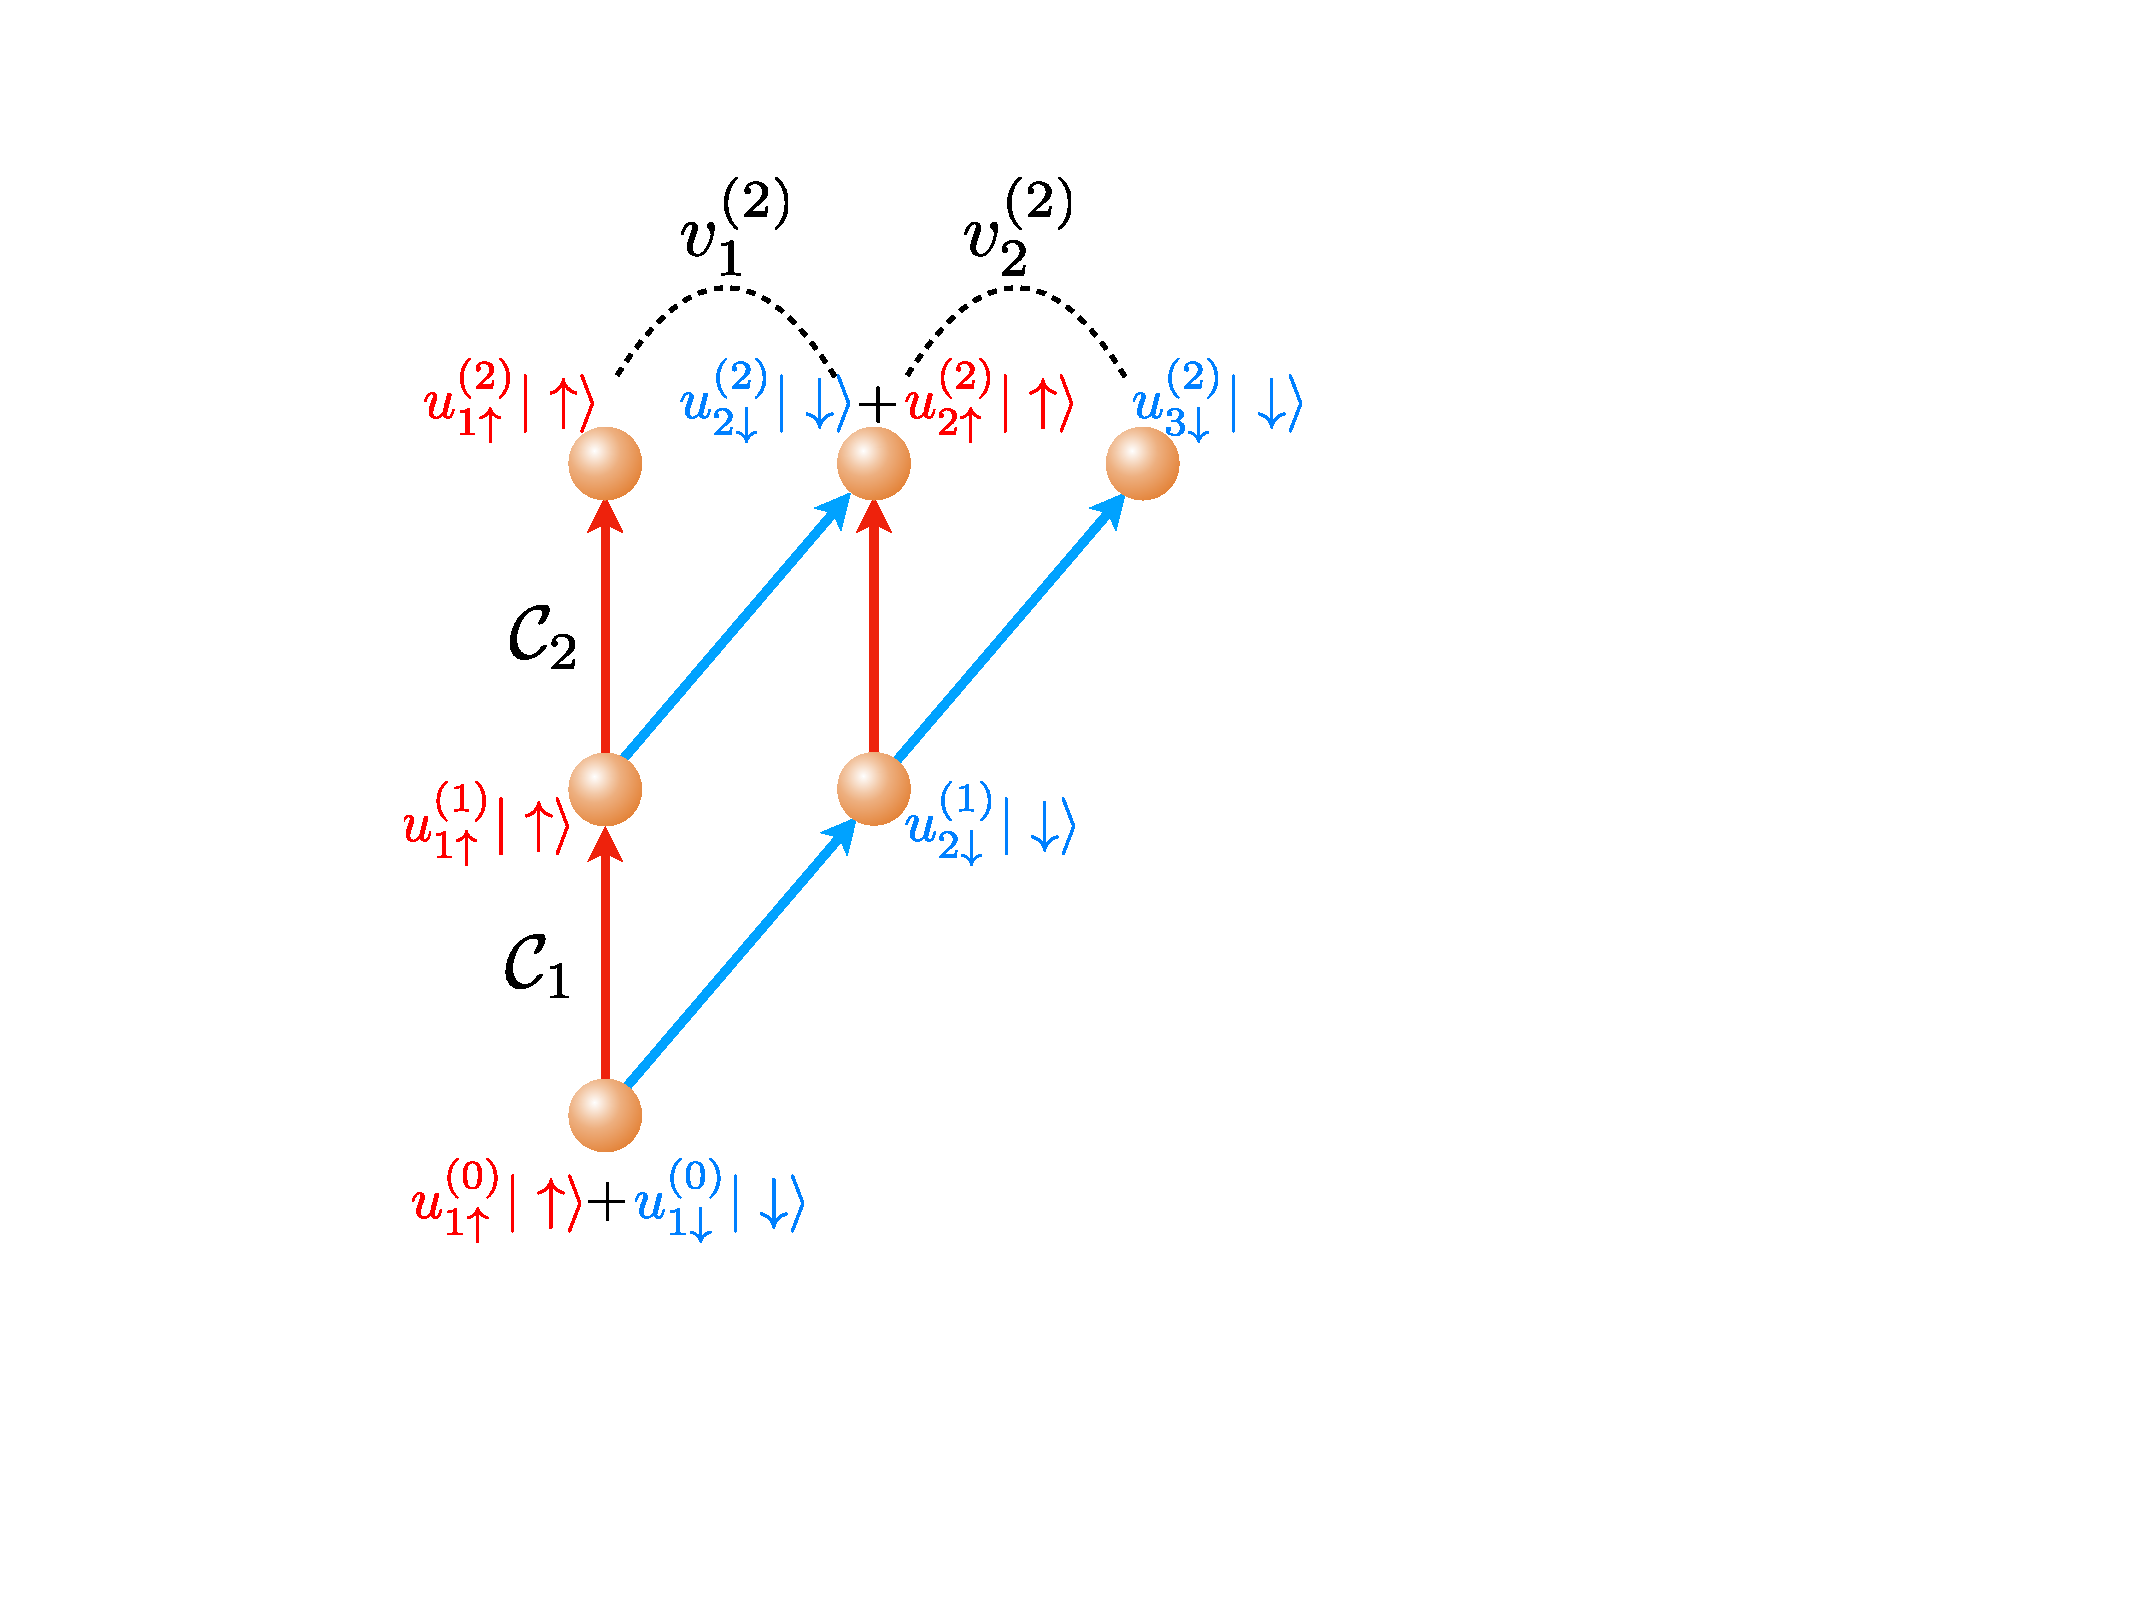
\includegraphics[width=0.3\columnwidth]{Scheme}
\caption{
    Schematic representation of how the amplitudes are distributed among the sites, at the various steps of the evolution.
    The red (blue) arrows represent the movement of the walker with coin state $\ket\uparrow$ ($\ket\downarrow$) after the coin flip.
    %It is clear from this representation why the ${u_{1,\downarrow} = u_{n+1, \uparrow} = 0}$ must hold.
    The coin operators $\mathcal C_i$ determine the weights with which the amplitude at every site is distributed between the red and blue arrows, and thus the two sites of the next layer with which it is connected.
}
\label{fig:QWs:conceptual_scheme_walker}
\end{figure}

An observation which will prove useful in~\cref{sec:QWs:reachability_conditions} is the way $\calS$ and $\calW_\calC$ act on the basis states $\ket{k,\uparrow},ket{k,\downarrow}$:
\begin{equation}
\begin{cases}
    \calS\ket{k,\uparrow} &= \ket{k,\uparrow}, \\
    \calS\ket{k,\downarrow} &= \ket{k+1, \downarrow},
\end{cases}
\qquad
\begin{cases}
    \calW_\calC\ket{k,\uparrow} &= c_{00} \ket{k,\uparrow} + c_{10} \ket{k+ 1,\downarrow}, \\
    \calW_\calC\ket{k,\downarrow} &= c_{01}\ket{k, \uparrow} + c_{11} \ket{k+1, \downarrow},
\end{cases}
\end{equation}
where we wrote the matrix elements of the coin operator as $(\calC)_{ij}=c_{ij}$.
We can moreover write more concisely the combined action of $\calC$ and $\calS$ by focusing on how $\calW$ acts on the single sites.
To see this, suppose that $\ket{\Phi}=\calW_\calC\ket{\Phi'}$ for some $\ket{\Phi},\ket{\Phi'}$ and $\calC$.
Then,
\begin{equation}
    \begin{pmatrix}
        \braket{k,\uparrow}{\Phi} \\
        \braket{k + 1, \downarrow}{\Phi}
    \end{pmatrix} =
    \calC \begin{pmatrix}
        \braket{k,\uparrow}{\Phi'} \\
        \braket{k,\downarrow}{\Phi'}
    \end{pmatrix},
    \qquad \forall k=1,...,n.
    \label{eq:QWs:dynamics_on_single_positions}
\end{equation}
We will also make use of an alternative way to represent states in $\calHwalker\otimes\calHcoin$ spanning $N$ sites, via two-column matrices. We write each state as a $N\times 2$ matrices in which each row contains the amplitudes associated with the corresponding site, and each column the amplitudes associated with a coin state.
We thus write $\ket\Psi$ as the $n\times2$ matrix
\begin{equation}
    \ket\Psi\doteq \begin{pmatrix}
        \Psi_{1,\uparrow} & \Psi_{1,\downarrow} \\
        \Psi_{2,\uparrow} & \Psi_{2,\downarrow} \\
        \multicolumn{2}{c}{\vdots} \\ 
        \Psi_{n,\uparrow} & \Psi_{n,\downarrow} \\
    \end{pmatrix}.
    \label{eq:QWs:matrix_notation}
\end{equation}
In this notation, the coin operation only introduces coherence between amplitudes on the same row, while the shift $\calS$ acts by shifting the second column downwards.

\begin{example}[label={ex:QWs:bimatrix_notation}]
    Here, we give explicit expressions for the states produced by a few steps of \ac{QW} evolution, using the matrix notation introduced in~\cref{eq:QWs:matrix_notation}. Let the initial state be $\ket{\Psi^{(0)}}\equiv\ket{1,\uparrow}$, and denote with $\calC_i$ be the coin operation at the $i$-th step, with elements $(\calC_i)_{jk}\equiv c^{(i)}_{jk}$.
    After a single step, we have
    \begin{equation}
        \ket{\Psi^{(1)}} =
        \begin{pmatrix}
            c^{(1)}_{11} & 0 \\
            0 & c^{(1)}_{21}
        \end{pmatrix}.
    \end{equation}
    After the second and third steps, we have
    \begin{equation}
        \ket{\Psi^{(2)}} =
        \begin{pmatrix}
            c^{(2)}_{11} c^{(1)}_{11} & 0 \\[0.4em]
            c^{(2)}_{12} c^{(1)}_{21} & c^{(2)}_{21} c^{(1)}_{11} \\[0.4em]
            0 & c^{(2)}_{22} c^{(1)}_{21} \\[0.4em]
        \end{pmatrix},
    \end{equation}
    \begin{equation}
        \ket{\Psi^{(3)}} =
        \begin{pmatrix}
            c^{(3)}_{11} c^{(2)}_{11} c^{(1)}_{11} & 0 \\[0.4em]
            c^{(3)}_{11} c^{(2)}_{12} c^{(1)}_{21} +
            c^{(3)}_{12} c^{(2)}_{21} c^{(1)}_{11} &
            c^{(3)}_{21} c^{(2)}_{11} c^{(1)}_{11} \\[0.4em]
            c^{(3)}_{12} c^{(2)}_{22} c^{(1)}_{21} &
            c^{(3)}_{21} c^{(2)}_{12} c^{(1)}_{21} +
            c^{(3)}_{22} c^{(2)}_{21} c^{(1)}_{11} \\[0.4em]
            0 & c^{(3)}_{22} c^{(2)}_{22} c^{(1)}_{21} \\[0.4em]
        \end{pmatrix}.
    \end{equation}
    While we do not give the explicit expressions for larger number of steps, we note how even from these first few expressions a very noticeable pattern emerges from the structure of the coefficients. For example, if we focus on the pedices of each element of these matrices, and read them from the right to the left, we get the following expression:
    \begin{equation}
        \begin{pmatrix}
            (11)(11)(11) & 0 \\
            (11)(12)(21) + (12)(21)(11) & (11)(11)(12) \\
            (12)(22)(21) & (11)(12)(22) + (12)(21)(12) \\
            0 & (12)(22)(22)
        \end{pmatrix},
    \end{equation}
    where the ``$+$'' symbols is here to be interpreted as a pure formal character, rather than as an actual sum. From this expression we can see how the following patterns emerge:
    \begin{itemize}
        \item Each sequence starts with a $1$ on the left, and ends with with a $1$ for the first column, or with a $2$ for the second column. The fact that each column starts with a $1$ is due to the initial coin state being $\ket\uparrow$, and would have been a $2$ if we instead started with $\ket\downarrow$.
        \item Between each pair of integers, the middle numbers are always identical (e.g. we never have something like $(11)(21)$). This is because each pair $(ij)$ represents the matrix component of a corresponding step changing the coin state from $i$ to $j$.
        \item In each entry, the number of $2$s on the right component of each pair equals the number of steps forward that the walker. For example, in the third row, we always have exactly two pairs with a $2$ on the right, consistently with the third row corresponding to output states of the form $\ket{3,\alpha}$.
    \end{itemize}
    These observations tell us that the initial and final number in each sequence, as well as the elements in between each pair, are redundant information. We can then represent the same state more efficiently by replacing each pair with its second element. We thus get
    \begin{equation}
        \begin{pmatrix}
            111 & 0 \\
            211 + 121 & 112 \\
            221 & 212 + 122 \\
            0 & 222
        \end{pmatrix}.
    \end{equation}
    This expression shows how finding the output amplitude corresponding to each one of the output modes is reduced to a purely combinatorial problem: starting with coin state $\ket\uparrow$ and evolving for $n$ steps, the output amplitude corresponding to the mode $\ket{k,s}$ with $s\in\{1,2\}$ has a number of contributions equal to the number of bitstrings of length $n$ that end with $s$ and have a number of $2$s equal to $k-1$.
    Once the set of bitstrings associated with a given output amplitude has been found, recovering the corresponding matrix elements of the coin operations, and thus the overall amplitude, is straightforward.

    As an example, suppose we are interested in knowing the amplitude associated with the walker evolving from $\ket{1,\uparrow}$ to $\ket{3,\downarrow}$ after $n=4$ steps. Following the above reasoning, we don't need to actually evolve the initial state through the associated unitary evolution matrices, but can instead immediately see that the amplitude is the one associated with the following four bitstrings:
    \begin{equation}
        1122, \quad 1212, \quad 2112,
    \end{equation}
    which are the possible bitstrings of four elements with two $2$s and ending with a $2$. The amplitude is therefore equal to
    \begin{equation}
        c^{(4)}_{22} c^{(3)}_{21} c^{(2)}_{11} c^{(1)}_{11} +
        c^{(4)}_{21} c^{(3)}_{12} c^{(2)}_{21} c^{(1)}_{11} +
        c^{(4)}_{21} c^{(3)}_{11} c^{(2)}_{12} c^{(1)}_{21}.
    \end{equation}
\end{example}


\section{Analytical results}
\label{sec:QWs:reachability_conditions}

In this section we provide a complete characterisation of the output states of time-dependent discrete-time \acp{QW} on a line.
We will find that such a characterisation can be formulated in terms of a sequence of efficiently verifiable conditions on the amplitudes of the output state.
More precisely, given a candidate output state, these conditions allow to (1) verify whether there is a sequence of coin operations generating the target states after the prescribed number of steps, and (2) if the answer is positive, obtain a possible such sequence.

\subsection{1-step reachability condition}
\label{sec:QWs:1step_reachability}

Let us start by analysing what happens for small numbers of steps. This will help to get intuition into the more general result.

Suppose the walker is initially localised at the site $i=1$ with some unspecified initial coin state $\ket\alpha$.
% $\ket s=u_{1,\uparrow}^{(0)}\ket{1,\uparrow} + u_{1,\downarrow}^{(0)}\ket{1,\downarrow}$.
The initial state of the full system is then written as
\begin{equation}
    \ket*{\Psi^{(0)}} \equiv
    \ket1\otimes\ket\alpha \equiv
    \ket{1}\otimes \big(u^{(0)}_{1,\uparrow} \ket{\uparrow} +
    u^{(0)}_{1,\downarrow} \ket{\downarrow} \big),
\end{equation}
denoting with $u^{(0)}_{1,\uparrow},u^{(0)}_{1,\downarrow}$ the amplitudes of $\ket\alpha$.
Let $\calC_1$ denote the coin operation performed at the first step,
and let $\calW_{\calC_1}$ be the corresponding step operation.
The state after the first step is then
$\ket*{\Psi^{(1)}} \equiv \calW_{\calC_1} \ket*{\Psi^{(0)}}$.
Explicitly, this reads
\begin{equation}
    \ket*{\Psi^{(1)}} =
    \calS \ket1\otimes(\calC_1\ket\alpha) =
    \mel{\uparrow}{\calC_1}{\alpha} \ket{1,\uparrow} +
    \mel{\downarrow}{\calC_1}{\alpha} \ket{2,\downarrow}.
\end{equation}
A notable feature of this state is that there are two vanishing amplitudes:
\begin{equation}
    \braket*{1, \downarrow}{\Psi^{(1)}} = \braket*{2, \uparrow}{\Psi^{(1)}} = 0.
\end{equation}
Note how this feature is independent on the initial coin state $\ket\alpha$ or the coin operation $\calC_1$, but is rather a general property of states produced by this kind of \ac{QW} dynamic.
More generally, for any initial walker state $\ket{\Psi}$ spanning $n$ sites, the application of $\mathcal W_{\mathcal C_1}$ produces a state spanning $n+1$ sites and satisfying the equations
\begin{equation}
	\mel{1, \downarrow}{\mathcal W_{\mathcal C_1}}{\Psi} =
	\mel{n+1, \uparrow}{\mathcal W_{\mathcal C_1}}{\Psi} = 0.
	\label{eq:QWs:vanishing_endpoints}
\end{equation}
This is a direct consequence of the structure of $\calS$, and can also be understood graphically from the pictorial representation in~\cref{fig:QWs:conceptual_scheme_walker}.
Indeed, the action of $\calS$ on an arbitrary state
$\ket\Psi\equiv\sum_{k=1}^N \sum_s \Psi_{k,s}\ket{k,s}$ reads
\begin{equation}
    \calS\ket\Psi =
    \sum_{k=1}^N (\Psi_{k,\uparrow}\ket{k,\uparrow} + \Psi_{k,\downarrow}\ket{k+1,\downarrow}),
\end{equation}
which means that $\mel{1,\downarrow}{\calS}{\Psi}=\mel{N+1,\uparrow}{\calS}{\Psi}=0$.
We can restate this result using the matrix notation introduced in~\cref{eq:QWs:matrix_notation} by saying that all and only the states that are the output of a step of \ac{QW} evolution have the form
\begin{equation}
    \begin{pmatrix}
        \bullet & 0 \\
        \bullet & \bullet \\
        \multicolumn{2}{c}{\vdots} \\ 
        \bullet & \bullet \\
        0 & \bullet \\
    \end{pmatrix},
    \label{eq:QWs:matrix_notation_vanishing_endpoints}
\end{equation}
where the $\bullet$ represent arbitrary amplitudes.
The implication goes both ways: any state $\ket\Phi$ of a system spanning $n+1$ sites and with an additional spin-like degree of freedom such that
$
\braket{1, \downarrow}{\Phi} =
\braket{n+1, \uparrow}{\Phi} = 0
$,
is the output of one step of a QW evolution with suitable coin operator and initial coin state.
To see this, suppose there are a coin operation $\calC$ and a state $\ket{\Phi'}$ such that $\calW_\calC\ket{\Phi'}=\ket{\Phi}$.
We then see from~\cref{eq:QWs:dynamics_on_single_positions} that any $\calC$ can be used, with a corresponding initial state $\ket{\Phi'}$ given by
\begin{equation}
    \begin{pmatrix}
        \Phi'_{k,\uparrow} \\
        \Phi'_{k,\downarrow}
    \end{pmatrix} = \calC^{-1}
    \begin{pmatrix}
        \Phi_{k,\uparrow} \\
        \Phi_{k+1,\downarrow}
    \end{pmatrix}
\end{equation}
We conclude that any state $\ket\Phi$ satisfying $\Phi_{1,\downarrow}=\Phi_{n+1,\uparrow}=0$ can be produced by a single step of a QW evolution.

\subsection{2-step reachability conditions}
\label{sec:QWs:2step_reachability}
We now consider the possible states after \textit{two} \ac{QW} steps.
Suppose $\ket\Psi$ spans $n+2$ modes and can be written as
$\ket\Psi=\calW_{\calC_2}\calW_{\calC_1}\ket*{\Psi^{(-2)}}$
for some unitaries $\calC_1,\calC_2$ and state $\ket*{\Psi^{(-2)}}$.
We will show in this section that all such states $\ket\Psi$ must satisfy a specific orthogonality condition on their amplitudes, and that, moreover, this condition, paired with the one discussed in~\cref{sec:QWs:1step_reachability}, is sufficient for a state $\ket\Psi$ to be output of two steps of a \ac{QW} dynamic.

From~\cref{sec:QWs:1step_reachability} we know that $\ket\Psi$ must be such that
$\Psi_{1,\downarrow}=\Psi_{n+2,\uparrow}=0$.
However, there is now an additional constraint to be taken into consideration. Namely, $\ket*{\Psi^{(-1)}}\equiv\calW_{\calC_1}\ket*{\Psi^{(-2)}}$ is also subject to the conditions derived in~\cref{sec:QWs:1step_reachability}:
$\Psi^{(-1)}_{1,\downarrow}=\Psi^{(-1)}_{n+1,\uparrow}=0$.
This constraint reflects on~\cref{eq:QWs:dynamics_on_single_positions}, which on the extremal sites now gives:
\begin{equation}
    \begin{pmatrix}
        \Psi_{1,\uparrow} \\
        \Psi_{2,\downarrow}
    \end{pmatrix} =
    \calC_1
    \begin{pmatrix}
        \Psi^{(-1)}_{1,\uparrow} \\
        \Psi^{(-1)}_{1,\downarrow}
    \end{pmatrix} =
    \calC_1
    \begin{pmatrix}
        \Psi^{(-1)}_{1,\uparrow} \\ 0
    \end{pmatrix},
\end{equation}
\begin{equation}
    \begin{pmatrix}
        \Psi_{n+1,\uparrow} \\
        \Psi_{n+2,\downarrow}
    \end{pmatrix} =
    \calC_1
    \begin{pmatrix}
        \Psi^{(-1)}_{n+1,\uparrow} \\
        \Psi^{(-1)}_{n+1,\downarrow}
    \end{pmatrix} =
    \calC_1
    \begin{pmatrix}
        0 \\
        \Psi^{(-1)}_{n+1,\downarrow}
    \end{pmatrix}.
\end{equation}
The unitarity of $\calC_1$ then directy implies that the length-$2$ vectors
$\begin{pmatrix}
    \Psi_{1,\uparrow} \\
    \Psi_{2,\downarrow}
\end{pmatrix}$
and
$\begin{pmatrix}
    \Psi_{n+1,\uparrow} \\
    \Psi_{n+2,\downarrow}
\end{pmatrix}$
are orthogonal\footnote{We are using here the characterisation of unitaries are those complex matrices whose rows (equivalently, columns) form an orthonormal system for the underlying vector space.}.
Let us then define the vectors $\bs v_j$ as:
\begin{equation}
    \bs v_j \equiv \begin{pmatrix}
        \Psi_{j,\uparrow} \\ \Psi_{j+1,\downarrow}
    \end{pmatrix},
    \qquad
    \bs v_j^{(-k)} \equiv \begin{pmatrix}
        \Psi^{(-k)}_{j,\uparrow} \\ \Psi^{(-k)}_{j+1,\downarrow}
    \end{pmatrix}.
\end{equation}
The orthogonality condition characterising $\Psi$ becomes
$
    \bs v_1^\dagger \bs v_{n+1} \equiv \langle \bs v_1, \bs v_{n+1}\rangle = 0,
$
which, together with~\cref{sec:QWs:1step_reachability}, gives the following two explicit conditions:
% \begin{subequations}
% 	\begin{align}
% 		u^{(2)}_{1, \downarrow} = u^{(2)}_{3, \uparrow} = 0,
% 		\label{eq:vanishing_endpoints_after_2steps}\\
% 		u^{(2)*}_{1, \uparrow} u^{(2)}_{2, \uparrow}
% 		+ u^{(2)*}_{2, \downarrow} u^{(2)}_{3, \downarrow} = 0.
% 		\label{eq:1st_orthogonality_condition}
% 	\end{align}
% 	\label[pluralequation]{eq:both_2ndstep_conditions}
% \end{subequations}
\begin{subequations}
 	% \label[pluralequation]{eq:both_2ndstep_conditions}
    \label{eq:QWs:both_2ndstep_conditions}
    \begin{align}
        \Psi_{1,\downarrow} = \Psi_{n+2,\uparrow} = 0,
 		\label{eq:QWs:vanishing_endpoints_after_2steps}\\
        \bar\Psi_{1,\uparrow} \Psi_{n+1,\uparrow} + 
        \bar\Psi_{2,\downarrow} \Psi_{n+2,\downarrow} = 0
 		\label{eq:QWs:1st_orthogonality_condition}
    \end{align}
\end{subequations}

Suppose now that $\ket\Phi$ is a state, spanning $n+2$ sites, and whose amplitudes satisfy~\cref{eq:QWs:both_2ndstep_conditions}.
Let $\ket*{\Phi^{(-1)}}$ be such that $\calW_{\calC_2}\ket*{\Phi^{(-1)}}$ for some $\calC_2$.
Then~\cref{eq:QWs:1st_orthogonality_condition}, remembering~\cref{eq:QWs:dynamics_on_single_positions}, implies that
$(\Phi^{(-1)}_{1,\uparrow},\Phi^{(-1)}_{1,\downarrow})^T$
is orthogonal to
$(\Phi^{(-1)}_{n+1,\uparrow},\Phi^{(-1)}_{n+1,\downarrow})^T$.
However, we want $\ket\Phi$ to be the output of \textit{two} steps, which means that we need $\ket*{\Phi^{(-1)}}$ to be a viable output of a single step. As per our conclusions from~\cref{sec:QWs:1step_reachability}, $\ket*{\Phi^{(-1)}}$ must therefore have the form~\cref{eq:QWs:matrix_notation_vanishing_endpoints}, which then forces the coin $\calC_2$ to be such that
\begin{equation}
    \begin{pmatrix}
        \Psi_{1,\uparrow} \\ \Psi_{2,\downarrow}
    \end{pmatrix} =
    \calC_2 \begin{pmatrix}
        a \\ 0
    \end{pmatrix},
    \qquad
    \begin{pmatrix}
        \Psi_{n,\uparrow} \\ \Psi_{n+1,\downarrow}
    \end{pmatrix} =
    \calC_2 \begin{pmatrix}
        0 \\ b
    \end{pmatrix}.
\end{equation}
Basic linear algebra then tells us that $\calC_2$ is forced to have the form
\begin{equation}
    \calC_2 = \begin{pmatrix}
        N_1 \Psi_{1,\uparrow} & N_2 e^{i\theta} \Psi_{n,\uparrow} \\
        N_1 \Psi_{2,\downarrow} & N_2 e^{i\theta} \Psi_{n+1,\downarrow}
    \end{pmatrix},
    \label{eq:QWs:coin_twosteps}
\end{equation}
where $N_1, N_2$ are normalisation constants to make the columns normalised, and $\theta\in\RR$ is an arbitrary phase.
It is worth noting that an additional phase factor could be added on the first column, but this would not make any difference to the physics, as it would amount to a global phase added to the unitary. In other words,~\cref{eq:QWs:coin_twosteps} determines an element of $\mathbf{U}(2)$ only up to its determinant\footnote{A more precise version of this statement is to say that we are determining the coins as elements of the quotient space $\mathbf{U}(2)/\mathbf U(1)\simeq\mathbf{SU}(2)$, in which matrices differing only by a multiplicative phase (equivalently, unitaries with different determinants), are considered as identical.}.
This choice of $\calC_2$ makes $\ket*{\Phi^{(-1)}}=\calW_{\calC_2}^{-1}\ket\Phi$ a possible outcome of a single step of \ac{QW} evolution.
Then, as per~\cref{sec:QWs:1step_reachability}, for any choice of $\calC_1$ we have that
$\calW_{\calC_1}^{-1}\calW_{\calC_2}^{-1}\ket\Phi$
is a state which after two steps produces the target $\ket\Phi$.


\subsection{3-step reachability conditions}
\label{sec:QWs:3step_reachability}
Let us now consider an output of three steps:
$\ket*{\Psi} \equiv \calW_{\calC_3}\calW_{\calC_2}\calW_{\calC_1} \ket*{\Psi^{(-3)}}$,
and assume that this state occupies $n+3$ position modes.
Then, denoting with
$\ket*{\Psi^{(-1)}} \equiv \calW_{\calC_2}\calW_{\calC_1} \ket*{\Psi^{(-3)}}$
the state at the previous step, we have that the amplitudes of $\ket*{\Psi^{(-1)}}$ must satisfy~\cref{eq:QWs:both_2ndstep_conditions}.
Here, these conditions have the form
$\bs v_1^{\dagger(-1)} \bs v_{n+1}^{(-1)}$,
which can be rewritten as
\begin{equation}
\begin{gathered}
	0 = \bs v_1^{\dagger(-1)} \bs v_{n+1}^{(-1)} = 
	\begin{pmatrix} \bar\Psi^{(-1)}_{1,\uparrow} & \bar\Psi^{(-1)}_{2,\downarrow} \end{pmatrix}
	\begin{pmatrix} \Psi^{(-1)}_{n+1,\uparrow} \\ \Psi^{(-1)}_{n+2,\downarrow} \end{pmatrix}
	\\
	=
	\begin{pmatrix} \bar\Psi^{(-1)}_{1,\uparrow} & \bar\Psi^{(-1)}_{1,\downarrow} \end{pmatrix}
	\begin{pmatrix} \Psi^{(-1)}_{n+1,\uparrow} \\ \Psi^{(-1)}_{n+1,\downarrow} \end{pmatrix} +
	\begin{pmatrix} \bar\Psi^{(-1)}_{2,\uparrow} & \bar\Psi^{(-1)}_{2,\downarrow} \end{pmatrix}
	\begin{pmatrix} \Psi^{(-1)}_{n+2,\uparrow} \\ \Psi^{(-1)}_{n+2,\downarrow} \end{pmatrix},
\end{gathered}
\end{equation}
where we used
$\Psi^{(-1)}_{1,\downarrow} = \Psi^{(-1)}_{n+2,\uparrow} = 0$.
Applying \cref{eq:QWs:dynamics_on_single_positions} on the above we get
\begin{equation}
\begin{aligned}
    \bs v_1^{\dagger} \calC_3 \calC_3^\dagger \bs v_{n+1}+
    \bs v_2^{\dagger} \calC_3 \calC_3^\dagger \bs v_{n+2}  =
    \bs v_1^{\dagger} \bs v_{n+1} +
    \bs v_2^{\dagger} \bs v_{n+2} = 0.
\end{aligned}
\label{eq:QWs:last_condition_for_psi3}
\end{equation}
Following a reasoning similar to the one used in the previous section, we conclude that the amplitudes of $\ket*{\Psi}$ satisfy three conditions:
the vanishing of the extremal amplitudes, $\bs v_1^{\dagger} \bs v_{n+2} = 0$, and~\cref{eq:QWs:last_condition_for_psi3}.

\subsection{Generalised reachability conditions}
\label{sec:QWs:general_reachability_conditions}

We analyse here the generalisation of the conditions derived in~\cref{sec:QWs:1step_reachability,sec:QWs:2step_reachability,sec:QWs:3step_reachability}, giving the conditions characterising states that can be the output of $m$ steps of some time-dependent QW.

Let $\ket\Psi$ be a state spanning $n+m$ sites, which is the output of at least $m$ steps of \ac{QW} evolution, so that
\begin{equation}
	\ket\Psi =
	\calW_{\calC_{m}} \calW_{\calC_{m-1}} ... \calW_{\calC_{1}}
    \ket{\Psi^{(0)}},
	\label{eq:QWs:starting_point}
\end{equation}
for some set of coin operators $\{\calC_i \}$ and initial state $\ket{\Psi^{(0)}}$.
Here, $\ket{\Psi^{(0)}}$ is an arbitrary state spanning $n$ positions (and which in particular is not required to satisfy any reachability condition of its own).
We want to show that, for any set of coin operators $\{\calC_i \}$, \cref{eq:QWs:starting_point} implies that $\ket\Psi$ satisfies the following conditions:
% \begin{equation}
\begin{gather}
	\Psi_{1,\downarrow} = \Psi_{n+m, \uparrow} = 0,
    \label{eq:QWs:vanishing_amplitudes}
	\\
    \sum_{i=1}^s \bs v_i^\dagger \bs v_{m+(n-1)-s+i} = 0,
	\text{ for } s=1,\ldots, m-1,
	\label{eq:QWs:orthogonality_conditions_for_vs}
\end{gather}
where $\bs v_{i}$ is again defined as
% \begin{equation*}
% 	\bs v_i \equiv
% 	\begin{pmatrix}
% 		\Psi_{i,\uparrow} \\ \Psi_{i+1, \downarrow}
% 	\end{pmatrix}.
% \end{equation*}
% \end{equation}
$\bs v_i \equiv (\Psi_{i,\uparrow}, \Psi_{i+1, \downarrow})^T$.
The cases $m=2$ and $m=3$ were worked out in~\cref{sec:QWs:2step_reachability,sec:QWs:3step_reachability},
so let us assume the statement to be true for $m$ and show that this implies it for $m+1$.
The main idea is to see how each one of the equations in \cref{eq:QWs:orthogonality_conditions_for_vs} transforms after one step.
Denote the amplitudes after a single step with $\Psi'_{i,\alpha}$.
The relation between primed and unprimed amplitudes is then
\begin{equation}
	\bs v_i^\prime
	= \mathcal C
	\begin{pmatrix}
		\Psi_{i,\uparrow} \\ \Psi_{i, \downarrow}
	\end{pmatrix},
	\text{ for each }
	i = 1, \dots, m,
	% \label{eq:evolution_amplitudes}
\end{equation}
for some unitary $\calC$,
where $\bs v'_i \equiv (\Psi_{i,\uparrow}',\Psi_{i+1,\downarrow}')^T$.
This directly implies, for all $i, j$,
\begin{equation}
	\begin{pmatrix}
		\bar\Psi_{i, \uparrow} & \bar\Psi_{i, \downarrow}
	\end{pmatrix}
	\begin{pmatrix}
		\Psi_{j, \uparrow} \\ \Psi_{j, \downarrow}
	\end{pmatrix}
	=
	\bs v^{\prime\dagger}_{i} \cdot \bs v^\prime_j.
    \label{eq:QWs:transition_us_to_vprimes}
\end{equation}
Explicitly, the $s$-th term in \cref{eq:QWs:orthogonality_conditions_for_vs} reads
\begin{equation}
	\bs v_1^\dagger \bs v_{m+n-s}
	+ \bs v_2^\dagger \bs v_{m+n-s+1}
	+ ...
	+ \bs v_{s-1}^\dagger \bs v_{m+n-2}
    + \bs v_s^\dagger \bs v_{m+n-1} = 0.
\end{equation}
Rewriting the LHS in terms of the amplitudes, rearranging the terms, and remembering that $\Psi_{1, \downarrow} = \Psi_{m+n, \uparrow} = 0$, we then get
\begin{equation}
\begin{aligned}
	\begin{pmatrix}
		\Psi_{1, \uparrow}^* & \Psi_{1, \downarrow}^*
	\end{pmatrix}
	\begin{pmatrix}
		\Psi_{m+n-s, \uparrow} \\ \Psi_{m+n-s, \downarrow}
	\end{pmatrix}
	+
	\begin{pmatrix}
		\Psi_{2, \uparrow}^* & \Psi_{2, \downarrow}^*
	\end{pmatrix}
	\begin{pmatrix}
		\Psi_{m+n-s+1, \uparrow} \\ \Psi_{m+n-s+1, \downarrow}
	\end{pmatrix} \\
	+ \cdots + 
	\begin{pmatrix}
		\Psi_{s, \uparrow}^* & \Psi_{s, \downarrow}^*
	\end{pmatrix}
	\begin{pmatrix}
		\Psi_{m+n-1, \uparrow} \\ \Psi_{m+n-1, \downarrow}
	\end{pmatrix}
	+
	\begin{pmatrix}
		\Psi_{s+1, \uparrow}^* & \Psi_{s+1, \downarrow}^*
	\end{pmatrix}
	\begin{pmatrix}
		\Psi_{m+n, \uparrow} \\ \Psi_{m+n, \downarrow}
	\end{pmatrix}.
\end{aligned}
\end{equation}
Using \cref{eq:QWs:transition_us_to_vprimes} we then get
\begin{equation}
	\bs v^{\prime\dagger}_1 \bs v^\prime_{m+n-s} +
	\bs v^{\prime\dagger}_2 \bs v^\prime_{m+n-s+1} +
	... +
    \bs v^{\prime\dagger}_{s} \bs v^\prime_{m+n-1} +
	\bs v^{\prime\dagger}_{s+1} \bs v^\prime_{m+n},
\end{equation}
or, equivalently,
$\displaystyle \sum_{i=1}^{s+1} \bs v^{\prime\dagger}_i \bs v^\prime_{m+n-(s+1)+i}=0$
for $s=1,\dots,m-1$.

\begin{figure}[tbh]
    \centering
    \begin{equation}
    \begin{pmatrix}
    \textcolor[rgb]{0.82,0.01,0.11}{\Psi _{1,\uparrow }} & 0\\
    \textcolor[rgb]{0.96,0.65,0.14}{\Psi _{2,\uparrow }} & \textcolor[rgb]{0.96,0.65,0.14}{\Psi }\textcolor[rgb]{0.96,0.65,0.14}{_{2,\downarrow }}\\
    \textcolor[rgb]{0.55,0.34,0.16}{\Psi _{3,\uparrow }} & \textcolor[rgb]{0.55,0.34,0.16}{\Psi }\textcolor[rgb]{0.55,0.34,0.16}{_{3,\downarrow }}\\
    \vdots  & \vdots \\
    \textcolor[rgb]{0.25,0.46,0.02}{\Psi _{m+n-1,\uparrow }} & \textcolor[rgb]{0.25,0.46,0.02}{\Psi }\textcolor[rgb]{0.25,0.46,0.02}{_{m+n-1,\downarrow }}\\
    0 & \textcolor[rgb]{0.56,0.07,1}{\Psi }\textcolor[rgb]{0.56,0.07,1}{_{m+n,\downarrow }}
    \end{pmatrix}\rightarrow \begin{pmatrix}
    \textcolor[rgb]{0.82,0.01,0.11}{\Psi '}\textcolor[rgb]{0.82,0.01,0.11}{_{1,\uparrow }} & 0\\
    \textcolor[rgb]{0.96,0.65,0.14}{\Psi '}\textcolor[rgb]{0.96,0.65,0.14}{_{2,\uparrow }} & \textcolor[rgb]{0.82,0.01,0.11}{\Psi '}\textcolor[rgb]{0.82,0.01,0.11}{_{2,\downarrow }}\\
    \vdots  & \textcolor[rgb]{0.96,0.65,0.14}{\Psi '}\textcolor[rgb]{0.96,0.65,0.14}{_{3,\downarrow }}\\
    \vdots  & \vdots \\
    \textcolor[rgb]{0.25,0.46,0.02}{\Psi '}\textcolor[rgb]{0.25,0.46,0.02}{_{m+n-1,\uparrow }} & \vdots \\
    \textcolor[rgb]{0.56,0.07,1}{\Psi '}\textcolor[rgb]{0.56,0.07,1}{_{m+n,\uparrow }} & \textcolor[rgb]{0.25,0.46,0.02}{\Psi '}\textcolor[rgb]{0.25,0.46,0.02}{_{m+n,\downarrow }}\\
    0 & \textcolor[rgb]{0.56,0.07,1}{\Psi '}\textcolor[rgb]{0.56,0.07,1}{_{m+n+1,\downarrow }}
    \end{pmatrix}
    \end{equation}
    \caption{
        Relation between $\ket\Psi$ and $\ket{\Psi'}\equiv\calW_\calC\ket\Psi$ as used in~\cref{sec:QWs:general_reachability_conditions}. The different colors correspond to pairs of amplitudes connected via $\calC$, as per~\cref{eq:QWs:dynamics_on_single_positions}.
    }
    \label{fig:QWs:visualisation_PsiVsPsip}
\end{figure}

This proves that, given $\ket\Psi$ satisfying~\cref{eq:QWs:orthogonality_conditions_for_vs}, any state of the form $\ket{\Psi'}=\calW_\calC\ket\Psi$ satisfies the $m-1$ constraints:
\begin{equation}
    \sum_{i=1}^{s} \bs v^{\prime\dagger}_i \bs v^\prime_{(m+1)+(n-1)-s+i}=0
	\text{ for }
	s = 2,...,m,
	\label{eq:QWs:general_orthogonality_almost_finished}
\end{equation}
which we can recognise as equivalent to~\cref{eq:QWs:orthogonality_conditions_for_vs} with $m\to m+1$, except for the $s=1$ condition, which amounts to $\bs v_1^{\prime\dagger}\bs v'_{(m+1)+n-1}=0$.
This last condition follows from $\Psi_{1,\downarrow}=\Psi_{n+m,\uparrow}=0$, as shown in~\cref{sec:QWs:2step_reachability}, and thus the induction step is completed.

In the special case of the initial state spanning a single position,~\cref{eq:QWs:orthogonality_conditions_for_vs} tells us that a state $\ket{\Psi}$ is a possible output of $n$ steps with initial state $\ket{1,\alpha}$ \textit{if and only} $\Psi_{1,\downarrow}=\Psi_{n+1,\uparrow}=0$, and the following $n-1$ conditions are met:
\begin{equation}
    \sum_{i=1}^s \bs v_i^{\dagger} \bs v_{n-s+i} = 0,
    \text{ for every } s=1,..,n-1.
    \label{eq:QWs:general_reachability_conditions}
\end{equation}

\begin{table}[tbh]
\centering
\begin{tabular}{cc@{\quad}l}
    \toprule
    \textbf{State} & \textbf{Occupied sites} & \textbf{Constraints} \\
    \midrule \\
    $\ket*{\Psi^{(0)}}$ & 1 & none \\
    \addlinespace[2pt]
    $\ket*{\Psi^{(1)}}$ & 2 & $u_{1,\downarrow} = u_{2,\uparrow} = 0$ \\
    \addlinespace[5pt]
    $\ket*{\Psi^{(2)}}$ & 3 &
    $\begin{dcases}
        u_{1,\downarrow} = u_{3,\uparrow} = 0 \\
        \bs v_1^{\dagger} \bs v_2 = 0
    \end{dcases}$ \\
    \addlinespace[5pt]
    % \addlinespace[0pt]\\
    $\ket*{\Psi^{(3)}}$ & 4 &
    $\begin{dcases}
        u_{1,\downarrow} = u_{4,\uparrow} = 0 \\
        \bs v_1^{\dagger} \bs v_3 = 0 \\
        \bs v_1^{\dagger} \bs v_2 + \bs v_2^{\dagger} \bs v_3 = 0
    \end{dcases}$ \\\addlinespace[4pt]
    \vdots & \vdots & \qquad\quad\vdots \\
    $\ket*{\Psi^{(n)}}$ & $n$+1 &
    $\begin{dcases}
        u_{1,\downarrow} = u_{n + 1,\uparrow} = 0 \\
        \sum_{i=1}^s \bs v_i^{\dagger} \bs v_{n-s+i} = 0
    \end{dcases}$ \\
    \bottomrule
\end{tabular}
\caption{
    Summary of the conditions characterising the states at the various stages of the evolution.
    For better clarity, we have avoided the use of superscripts on the amplitudes.
The amplitudes in each row refer to the corresponding state at that step.
    The conditions shown in the case $\ket*{\Psi^{(n)}}$ hold for all $s=1,..., n-1$, consistently with~\cref{eq:QWs:general_reachability_conditions}.
}
\label{table:QWs:constraints}
\end{table}

\begin{example}[label=ex:QWs:conditions_few_steps]
    To illustrate how the derived conditions work, consider an example with initial state
    \begin{equation}
        \ket{\Psi} = \frac{1}{\sqrt4} (
        \ket{1,0} + \ket{2,+} + \ket{3, -} + \ket{4, 1}
        ).
    \end{equation}
    Let $\calC_1=H$, with $H$ the Hadamard matrix, which satisfies
    \begin{equation}
        H\ket0=\ket+, \quad H\ket1=\ket-,
        \quad H\ket+=\ket0, \quad H\ket-=\ket1.
    \end{equation}
    Follow the matrix notation introduced in~\cref{eq:QWs:matrix_notation}, we have
    \begin{equation}
        \ket{\Psi} \simeq
        \frac{1}{\sqrt4}
        \begin{pmatrix}
            1 & 0 \\
            1/\sqrt2 & 1/\sqrt2 \\
            1/\sqrt2 & -1/\sqrt2 \\
            0 & 1
        \end{pmatrix}
    \end{equation}
    Because this state satisfies the conditions given in~\cref{sec:QWs:1step_reachability} about the vanishing endpoints, $\Psi_{1,\downarrow}=\Psi_{4,\uparrow}=0$, we know that this is a possible output of a single step. On the other hand, it does not satisfy the conditions given in~\cref{sec:QWs:2step_reachability} to be the output of \textit{two} steps.
    Consider now the evolved state $\ket{\Psi'}\equiv\calW_{\calC_1}\ket\Psi$ with $\calC_1\equiv H\equiv\frac{1}{\sqrt2}(I+Z)$ the Hadamard matrix. In matrix notation, this will be
    \begin{equation}
        \ket{\Psi'} =
        \frac{1}{\sqrt4}
        \begin{pmatrix}
            1/\sqrt2 & 0 \\
            1 & 1/\sqrt2 \\ 
            0 & 0 \\
            1/\sqrt2 & 1 \\
            0 & -1/\sqrt2
        \end{pmatrix}.
        \label{eq:QWs:example_psi'}
    \end{equation}
    The vectors $\bs v'$ then equal $\bs v'_1=(1/\sqrt2, 1/\sqrt2)$ and
    $\bs v'_4=(1/\sqrt2, -1/\sqrt2)$,
    which are clearly orthogonal, again consistently with $\ket{\Psi'}$ being output of two steps.
    Let us consider an additional step, with coin $\calC_2=\frac{1}{\sqrt2}(I + iX)$.
    Writing the output with $\ket{\Psi''}=\calW_{\calC_2}\ket{\Psi'}$, we have
    \begin{equation}
        \ket{\Psi''} = \frac{1}{4}
        \begin{pmatrix}
            1 & 0 \\
            i + \sqrt2 & i \\
            0 & 1 + i\sqrt2 \\
            1 + i\sqrt2 & 0 \\
            -i & i + \sqrt2 \\
            0 & -1
        \end{pmatrix}.
    \end{equation}
    The relevant $\bs v''$ vectors are for this state
    \begin{equation}
    \begin{aligned}
        &\bs v''_1 = \frac{1}{4}\begin{pmatrix} 1 \\ i \end{pmatrix},
        &&\bs v''_2 = \frac{1}{4}\begin{pmatrix} \sqrt2 + i \\ 1 + i\sqrt2 \end{pmatrix}, \\
        &\bs v''_4 = \frac{1}{4}\begin{pmatrix} 1 + i\sqrt2\\ \sqrt2 + i \end{pmatrix},
        &&\bs v''_5 = \frac{1}{4}\begin{pmatrix} -i \\ -1 \end{pmatrix},
    \end{aligned}
    \end{equation}
    It is then straightforward to verify that
    $\bs v_1^{\dprime\dagger}\bs v_5'' = 0$.
    Furthermore,
    $\bs v_1^{\dprime\dagger}\bs v_4'' = 1/8$
    and $\bs v_2^{\prime\prime\dagger}\bs v_5'' = -1/8$,
    thus 
    $\bs v_1^{\dprime\dagger}\bs v_4'' + \bs v_2^{\dprime\dagger}\bs v_5'' = 0$,
    again consistently with the results of~\cref{sec:QWs:3step_reachability}.
    As a last remark, let us show how we would go in recovering the coin operators generating $\ket{\Psi''}$, assuming we are only given this state without further knowledge.
    The idea behind such reconstruction is to observe that if $\tilde\calC_1$ is such that $\calW_{\tilde\calC_1}\ket{\Phi'}=\ket{\Psi''}$ for some $\ket{\Phi'}$, then, from~\cref{eq:QWs:dynamics_on_single_positions}, we know that $\tilde\calC_1^\dagger \bs v_1''\simeq(1,0)^T$ and $\tilde\calC_1^\dagger \bs v_5''\simeq(0,e^{i\phi})^T$ for some $\phi_1\in\RR$. It follows that
    \begin{equation}
        \tilde\calC_1 =
        % \begin{pmatrix}
        %     N_1 \bs v_1'' & N_2 e^{i\phi} \bs v_5''
        % \end{pmatrix} = \frac{1}{\sqrt2}
        \frac{1}{\sqrt2} \begin{pmatrix}
            1 & e^{i\phi_1}i \\
            i & e^{i\phi_1}1
        \end{pmatrix}.
    \end{equation}
    This is clearly consistent with the coin we used being $\frac{1}{\sqrt2}(I+iX)$, but also shows that multiple initial states are compatible with the output, thanks to the freedom in choosing $\phi_1$. The corresponding $\ket{\Phi'}$ are then
    \begin{equation}
        \ket{\Phi'} = \frac{1}{2\sqrt2}
        \begin{pmatrix}
            1 & 0 \\
            \sqrt2 & e^{-i\phi_1} \\
            0 & 0 \\
            1 & \sqrt2 e^{-i\phi_1} \\
            0 & -e^{-i\phi_1}
        \end{pmatrix},
    \end{equation}
    consistently with~\cref{eq:QWs:example_psi'}.
    Going further back, we use $\bs v_1'\simeq(1,e^{-i\phi_1})^T$ and $\bs v_4'\simeq(1,-e^{-i\phi_1})^T$ to find the previous possible coins $\tilde\calC_2$ to be of the form
    \begin{equation}
        \tilde\calC_2 = \frac{1}{\sqrt2} \begin{pmatrix}
            1 & e^{i\phi_2} \\
            e^{-i\phi_1} & -e^{i(\phi_2-\phi_1)}
        \end{pmatrix},
    \end{equation}
    for all $\phi_2\in\RR$. The reconstructed initial state $\ket\Phi$ is then found to have the form
    \begin{equation}
        \ket\Phi = \frac{1}{2\sqrt2}
        \begin{pmatrix}
            \sqrt2 & 0 \\
            1 & e^{-i\phi_2} \\
            1 & -e^{-i\phi_2} \\
            0 & \sqrt2 e^{-i\phi_2}
        \end{pmatrix}.
    \end{equation}
    An interesting feature emerging from this example is that the freedom in the choice of the coin operations does not ``cumulate'', in the sense that the possible states producing a target after a number of steps are still uniquely defined up to only a phase difference between the two coin states.
\end{example}

\subsection{Find coin operators generating a state}
\label{sec:QWs:coin_operators_generating_state}

\tmpHeading{Goal of the section}
In~\cref{sec:QWs:reachability_conditions} we showed that, if $\ket\Psi=\calW_{\calC_n}\cdots\calW_{\calC_1}\ket{\Psi_{\on{in}}}$, then the amplitudes of $\ket\Psi$ must satisfy the conditions given in~\cref{eq:QWs:general_reachability_conditions}.
Here we show that also the opposite holds: given a state $\ket\Psi$ satisfying~\cref{eq:QWs:general_reachability_conditions}, there is always a choice of coin operations $\calC_i$ and initial state $\ket{\Psi_{\on{in}}}$ that produce $\ket\Psi$.

\tmpHeading{Vanishing amplitudes imply state is output of one step}
Suppose that a state $\ket\Psi$ over $n$ sites satisfies $\Psi_{1,\downarrow}=\Psi_{n,\uparrow}=0$. Then, for any choice of unitary coin operator $\calC$, there is some $\ket{\Psi'}$ such that $\ket\Psi=\calW_\calC\ket{\Psi'}$.
This is straightforward, as $\calW_\calC\ket{\Psi'}$ will always have vanishing extremal amplitudes, regardless of $\calC$. For a given choice of $\calC$, the initial state $\ket{\Psi'}$ is uniquely determined by $\ket{\Psi'}=\calW_\calC^{-1}\ket\Psi$.

\tmpHeading{Reconstructing coin operators after \emph{two} steps}
Suppose now that $\ket\Psi$, on top of $\Psi_{1,\downarrow}=\Psi_{n,\uparrow}=0$, also satisfies $\bs v_1^\dagger \bs v_{n-1}=0$. Then, if $\ket\Psi=\calW_\calC\ket{\Psi'}$, we must have
$\bs v_1=\calC(\Psi'_{1,\uparrow},\Psi'_{1,\downarrow})^T$ and
$\bs v_{n-1}=\calC(\Psi'_{n-1,\uparrow},\Psi'_{n-1,\downarrow})^T$,
with $(\Psi'_{1,\uparrow},\Psi'_{1,\downarrow})$ orthogonal to
$(\Psi'_{n-1,\uparrow},\Psi'_{n-1,\downarrow})$.
Because we already shown that $\ket{\Psi'}=\calW_{\calC'}\ket{\Psi''}$ for some $\calC'$ and $\ket{\Psi''}$ if and only if the extremal amplitudes vanish, we know that, for $\ket\Psi$ to be output of \emph{two} steps of QW, its amplitudes must satisfy
$\Psi'_{1,\downarrow}=\Psi'_{n-1,\uparrow}=0$. This, in turn imposes a constraint on $\calC$, which must be a unitary such that
\begin{equation}
    \bs v_1 = \calC \begin{pmatrix}
        \Psi'_{1,\uparrow} \\ 0
    \end{pmatrix}, \qquad
    \bs v_{n-1} = \calC \begin{pmatrix}
        0 \\ \Psi'_{n-1,\downarrow}
    \end{pmatrix}.
\end{equation}
This implies that $\calC'$ must be a unitary whose columns equal, up to normalisation, $\bs v_1$ and $\bs v_{n-1}$. Note that a phase can also be added to each column independently without affecting these relations. Remembering that unitaries differing only by a global phase are effectively equivalent, we can write the set of viable coin operators as
$\calC = (\bs v_1^T/\|\bs v_1\|, e^{i\phi}\bs v_{n-1}^T/\|\bs v_{n-1}\|)$,
for some $\phi\in\RR$.
We thus conclude that, for any such $\calC$, we have $\ket{\Psi'}\equiv\calW_{\calC}^{-1}\ket\Psi$ such that $\Psi'_{1,\downarrow}=\Psi'_{n-1,\uparrow}=0$, and thus for any choice of $\calC'$ there is also some $\ket{\Psi''}$ such that $\ket\Psi=\calW_\calC\calW_{\calC'}\ket{\Psi''}$.

\tmpHeading{Reconstructing coin operators after \emph{three} steps}
The next step is to consider what happens when $\ket\Psi$ satisfies, on top of the two conditions used in the previous paragraph, also
\begin{equation}
    \bs v_1^\dagger \bs v_{n-2}+\bs v_2^\dagger \bs v_{n-1}=0.
    \label{eq:QWs:orthogonality_on_vs_proving_otherdirection}
\end{equation}
The argument in the previous paragraphs can be used to find $\ket{\Psi'},\ket{\Psi''},\calC,\calC'$ such that
$\ket\Psi=\calW_\calC\ket{\Psi'}=\calW_\calC\calW_{\calC'}\ket{\Psi''}$.
We now observe that $\ket{\Psi'}=\calW_{\calC'}\ket{\Psi''}$ implies
\begin{equation}
    \bs v_1^\dagger \bs v_{n-2}+\bs v_2^\dagger \bs v_{n-1} =
    % \bar\Psi_{1,\uparrow}\Psi_{n-2,\uparrow} + \bar\Psi_{3,\downarrow}\Psi_{n,\downarrow} =
    \bs v_1'^\dagger \bs v_{n-2}' = 0.
\end{equation}
But this now implies that $\ket{\Psi'}$ can be the output of \emph{two} steps, and therefore the existence of $\calC''$ and $\ket{\Psi'''}$ such that
$\ket\Psi=\calW_\calC\calW_{\calC'}\calW_{\calC''}\ket{\Psi'''}$.
The coin operators $\calC,\calC'$ are again determined as those whose columns equal $\bs v_1,\bs v_{n-1}$ and $\bs v_1',\bs v_{n-2}'$, respectively. Arbitrary phase differences $\phi_1,\phi_2$ can be introduced between the columns of $\calC,\calC'$, but it is worth noting that the phase difference introduced in $\calC$ will affect the choice of $\calC'$ in such a way that $\ket{\Psi'''}$ will \emph{not} be dependent on it.
We refer to~\cref{ex:QWs:conditions_few_steps} for a detailed practical example of deriving such coin operators.

\tmpHeading{General case}
The general case of $\ket\Psi$ satisfying
\begin{equation}
    \sum_{i=1}^s \bs v_i^\dagger \bs v_{m-1-s+i}=0
    \text{ for all }s=1,...,\ell-1
    \label{eq:QWs:orthogonality_conditions_vs_inverse_proof_section}
\end{equation}
is fully analogous. We start by using $\bs v_1^\dagger \bs v_{n-1}=0$ to find a coin $\calC$ such that $\ket{\Psi'}=\calW_{\calC}^{-1}\ket\Psi$ has vanishing extremal amplitudes. We then observe that the amplitudes of such $\ket{\Psi'}$ must also satisfy~\cref{eq:QWs:orthogonality_conditions_vs_inverse_proof_section} with $m\to m-1$ and $\ell\to\ell-1$, and thus iterate the reasoning.



% We conclude our analysis of the global reachability conditions by remarking that \cref{eq:QWs:general_reachability_conditions} completely characterises the set of quantum states reachable after $n$ steps.
% In other words, not only every state that is the result of a \ac{QW} evolution satisfies it, but also for every state $\ket*{\Phi}$ that satisfies \cref{eq:QWs:general_reachability_conditions}, there is a set of coin operators $\{ \mathcal C_i \}_{i=1}^n$ and an initial state $\ket{\Phi_{in}}$ such that
% $\ket\Phi = 
%     \mathcal W_{\mathcal C_n} \cdots \mathcal W_{\mathcal C_1}
%     \ket{\Phi_{in}}$.
% In fact, given the state $\ket\Phi$, this set of coin operators is efficiently computable.
% This was already sketched in a previous section, but we will here give a more detailed and general description of the computation.

% We start by noting that,
% denoting with $\bs v_i$ the $\bs v$-vectors built from the amplitudes of a generic $\ket{\Phi}$ satisfying~\cref{eq:QWs:general_reachability_conditions}, we have $\bs v_1^\dagger \bs v_n = 0$.
% This immediately implies the existence of a $2\times2$ unitary matrix $\calC_n$, and complex numbers $a$ and $b$, such that
% \begin{equation}
%     \bs v_1 = \mathcal C_n
%     \begin{pmatrix} a \\ 0 \end{pmatrix},
%     \qquad
%     \bs v_n = \mathcal C_n
%     \begin{pmatrix} 0 \\ b \end{pmatrix}.
%     \label{eq:equations_giving_C}
% \end{equation}
% The first of the above equations implies that the second row of $\mathcal C_n^{-1}$ is orthogonal to $\bs v_1$, that is,
% % \begin{equation}
% $
%     - c_{21} u_{1, \uparrow} + c_{11} u_{2, \downarrow} = 0.
% $
% This condition is enough, together with the constraint of the columns of a unitary matrix being normalised, to determine the first column of $\mathcal C_n$ up to a phase.
% The orthonormality constraint that $\mathcal C_n$ must satisfy then determines the elements of the second column, again up to a phase.
% This leaves the freedom to choose two different phases for the two columns.
% Finally, remembering that the global phase of $\mathcal C_n$ does not have physical consequences, we conclude that $\mathcal C_n$ is determined up to a phase difference between the two columns.
% More explicitly, the above argument tells us that the coin operators generating a walker state spanning $n+1$ sites are all and only the unitaries of the form
% \begin{equation*}
% \begin{aligned}
%     \mathcal C_n
%     &= N \begin{pmatrix}
%         u_{1,\uparrow} & e^{i\alpha} u_{\makebox[0pt][l]{$\scriptstyle n$}\phantom{n+1},\uparrow} \\
%         u_{2,\downarrow} & e^{i\alpha} u_{n+1,\downarrow}
%     \end{pmatrix} = N \begin{pmatrix}
%         u_{1,\uparrow} & -e^{i\alpha} u_{2,\downarrow}^* \\
%         u_{2,\downarrow} & \phantom{-}e^{i\alpha} u_{1,\uparrow}^*
%     \end{pmatrix},
% \end{aligned}
% \end{equation*}
% with $\alpha$ arbitrary and $N$ normalisation constant.
% This coin operator can then be written, using for example the parametrization of~\cite{chandrashekar2008optimizing}, as
% \begin{equation}
%     \mathcal C_n = 
%     \begin{pmatrix}
%         e^{i\xi} \cos\theta &
%         e^{i\zeta} \sin\theta \\
%         -e^{-i\zeta}\sin\theta & e^{-i\xi}\cos\theta
%     \end{pmatrix},
%     \label{eq:su2_coin_matrix}
% \end{equation}
% with $\theta\in [0, \pi/2]$, $\xi$ and $\zeta$ satisfying
% $\tan\theta = \lvert u_{2,\downarrow} \rvert/\lvert u_{1,\uparrow} \rvert$
% and
% $\xi + \zeta \pm \pi = \arg\left(u_{1, \uparrow}/u_{2, \downarrow}\right)$.
% The freedom in $\alpha$ is here translated into the phase difference $\zeta - \xi$ not being uniquely determined.
% More explicitly, when tracing back the evolution of the walker one can at every step write the coin operator as in \cref{eq:su2_coin_matrix} with $\xi \to \xi + \varphi$ and $\zeta \to \zeta - \varphi$ for an arbitrary $\varphi\in \mathbb R$.
% Trivial modifications must be applied to the above formulae when $u_{2,\downarrow} = 0$.

% To obtain the coin operators at the previous steps, we use the $\mathcal C_n$ computed above to get the amplitudes of $\mathcal W_{\mathcal C_n}^{-1} \ket\Phi$.
% These amplitudes will again satisfy the orthogonality condition between the $\bs v$-vectors at the first and last sites:
% ${\bs v_1^\dagger \bs v_{n-1} = 0}$
% (where now $\bs v_i$ refers to the amplitudes after the $(n-1)$-th step).
% The same argument used above can now be repeated, to compute the coin operator at this step.
% Iterating this procedure we can compute all of the coin operators, with the exception of the first one.
% In fact, the amplitudes after the first step do not satisfy the orthogonality condition like \cref{eq:equations_giving_C} anymore (the only condition on them is the vanishing of the extremal amplitudes), so that the above argument breaks.
% This last (first) coin operator is nevertheless easily solved for by remembering that the only non vanishing amplitudes at this stage of the evolution are $u_{1,\uparrow}$ and $u_{2, \downarrow}$, so that if the initial state is
% ${\ket{\Phi_{in}} = u^{(0)}_{1,\uparrow} \ket{1, \uparrow} + u^{(0)}_{1, \downarrow} \ket{1, \downarrow}}$, then the first coin operator must satisfy
% \begin{equation}
%     \begin{pmatrix}
%         u_{1, \uparrow} \\ u_{2,\downarrow}
%     \end{pmatrix}
%     = \mathcal C_1
%     \begin{pmatrix}
%         u^{(0)}_{1, \uparrow} \\ u^{(0)}_{1, \downarrow}
%     \end{pmatrix}.
% \end{equation}
% The values of $u_{1, \uparrow}, u_{2,\downarrow}, u^{(0)}_{1, \uparrow}$ and $u^{(0)}_{1, \downarrow}$ are known, so that this equation is readily solved for the elements of $\mathcal C_1$, for any initial state $\ket{\Phi_{in}}$.


% \subsection{Dimension of space of reachable states}
% \label{sec:QWs:reachable_space}

% Given the full characterisation of outputs of~\acp{QW}, a natural next question is: \textit{fixing a number of steps $n$, what portion of the space of $n\times 2$-dimensional states can be obtained with this kind of dynamic?}
% The set of all (pure) states over $n+1$ sites and with a two-dimensional coin is a $[2\times2(n+1)-2]=(4n+2)$-dimensional real manifold (more precisely, this is the complex projective space $\mathbb{CP}^{2n+1}$).

% The total number of (real) degrees of freedom of a walker state after $n$ steps, considering the two vanishing extremal amplitudes, is $4n - 2$.
% Additionally, the set of constraints in \cref{eq:QWs:general_reachability_conditions} amounts to $2(n-1)$ real conditions.
% It follows that the space of reachable states $\ket*{\Psi^{(n)}}$ has dimension $2n$, to compare with the number of degrees of freedom of a general state living in the same Hilbert space, that is, $4n + 2$.
% This is consistent with the fact that 
%Note how this is consistent with our finding that when computing the coin operator generating a state, the phase difference between its columns can be freely chosen. Therefore, the number of parameters characterising all the possible SU(2) coin operators for $n$ steps is $2n$, being each coin operator characterised by only two parameters.


\section{Focusing on walker states}
\label{sec:QWs:focusing_walker_states}

In~\cref{sec:QWs:reachability_conditions} we characterised the states that can be generated via \acp{QW}.
Here, we consider the scenario in which one is interested in generating a target \emph{qudit} state over the walker's degree of freedom, as opposed to a target in the full walker and coin space.
In other words, we fix a number of steps $n$ and a target superposition over the sites $\ket\phi=\sum_{i=1}^{n+1} u_i\ket i$, and ask whether there is a combination of coins $\{\calC_i\}_{i=1}^{n}$, a final coin state $\ket\gamma$, and an initial state $\ket{\Psi_0}=\ket{1, \alpha}$ for some initial coin state $\ket\alpha$, such that, up to a normalisation factor,
\begin{equation}
    \mel{\gamma}{\calW_{\calC_{n}} \cdots\calW_{\calC_{1}}}{\Psi_0} = \ket\phi.
\end{equation}
Such protocols are clearly probabilistic in general, but this is not a big hurdle provided the projection probabilities are vanishingly small.
In particular, we are interested in finding whether arbitrary $\ket\phi$ can be generated in this way.
The main tool that will be used to answer this question are the results of~\cref{sec:QWs:reachability_conditions}.
We will find the answer to be positive, modulo a few degenerate conditions that the $\ket\phi$ need to satisfy.
For the analytical results, we focus on the case of the coin being projected over $\ket+$,
and provide numerical results for the more general case.

Let $\ket\phi$ be an arbitrary superposition of $n+1$ sites with amplitudes $u_k \equiv \braket{k}{\phi}$.
We want to find a reachable walker state $\ket\Phi$, in the full walker and coin space, such that
$\ket{+}_c \!\!\!\!\braket{+}{\Phi} \propto \ket\phi \!\otimes\! \ket+$.
Denoting with $\Phi_{i,s}$ the amplitudes of $\ket\Phi$, this amounts to finding a $\ket\Phi$ whose amplitudes simultaneously satisfy, on top of the reachability conditions of~\cref{eq:QWs:general_reachability_conditions}, the relations
${N(\Phi_{i,\uparrow}+\Phi_{i,\downarrow})= u_i}$ for all $i$.
In order to do this, we parametrize the set of all walker states $\ket\Phi$ whose amplitudes give the target after projection as
\begin{equation}
\begin{aligned}
    \ket\Phi &= N^{-1/2} \left( u_1 \ket{1,\uparrow} + u_{n+1} \ket{n+1,\downarrow}
	+ \sum_{i=2}^n \left[
		(u_i - d_i) \ket{i, \uparrow} +
		d_i \ket{i, \downarrow}
	\right] \right),
\end{aligned}
\label{eq:QWs:parametrized_state_with_ds}
\end{equation}
where $(d_i)_{i=2}^n$ are complex parameters to be determined, and $N\in\RR$ ensures the normalisation.
Projecting \cref{eq:QWs:parametrized_state_with_ds} over the coin state $\ket+$ gives the correct result for any choice of $d_i$.
The problem is thus reduced to finding $(d_i)_{i=2}^n$ corresponding to a reachable state.
If a set of coefficients is then found to generate the target state, the associated projection probability is computed as
$\|\braket{+_c}{\Phi}\|^2=1/2N$.
From~\cref{sec:QWs:reachability_conditions}, we know that $\ket\Phi$ is reachable \textit{if and only if}~\cref{eq:QWs:general_reachability_conditions} is satisfied. Together with~\cref{eq:QWs:parametrized_state_with_ds} these conditions translate into $\sum_{i=1}^{s} \bs v_i^\dagger \bs v_{n-s+i}=0$ for all $s=1,\dots,n-1$, where
\begin{equation}
    \bs v_i \equiv \begin{pmatrix}
        u_i - d_i \\ d_{i+1}
    \end{pmatrix},
    \text{ with } d_1 = 0 \text{ and } d_{n+1}=u_{n+1}.
\end{equation}
Explicitly, we then get the following conditions on the parameters $d_i$:
\begin{equation}
	\sum_{i=1}^s \left[
	  (u_i - d_i)^*
      (u_{i+(n-s)} - d_{i+(n-s)})
	  +
      d_{i+1}^* d_{i+(n-s)+1}
    \right]
	= 0,
	\label{eq:QWs:conditions_for_ds}
\end{equation}
for every $s=1,\dots,n-1$,
with $d_1=0$ and $d_{n+1}=u_{n+1}$.
Isolating the unknowns from the rest of the parameters, we rewrite~\cref{eq:QWs:conditions_for_ds} as
\begin{equation}%\footnotesize
\begin{aligned}
    2\sum_{i=2}^s d_i^* d_{i+(n-s)}
    + \sum_{i=1}^s u_i^* u_{i+(n-s)} \\
    - \sum_{i=n-s+1}^{n} u_{i-(n-s)}^* d_i
    - \sum_{i=2}^{s} u_{i+(n-s)} d_i^*
    + u_{n+1} d_{s+1}^* 
    = 0.
\end{aligned}
\end{equation}
If we then define
\begin{equation}
\begin{gathered}
    Q_s \equiv 2\sum_{i=2}^s \ketbra{i}{i+(n-s)},
    \qquad
    C_s \equiv \sum_{i=1}^s u_i^* u_{i+(n-s)},
    \qquad
    \tilde{\bs d} \equiv (\bs d, 1)^T, \\
    \bs\alpha_s \equiv -\sum_{i=1+(n-s)}^n u_{i-(n-s)}\ket{i},
    \qquad
    \bs\beta_s \equiv -\sum_{i=2}^{s} u_{i+(n-s)}\ket{i} + u_{n+1} \ket{s+1},
\end{gathered}
\end{equation}
we conclude that the reachability is equivalent to the following system of complex quadratic equations:
\begin{equation}
    \tilde{\bs d}^\dagger
    \begin{pmatrix}
        Q_s & \bs\beta_s \\
        \bs\alpha_s^\dagger & C_s
    \end{pmatrix}
    \tilde{\bs d} = 0.
\end{equation}
This shows that the conditions in~\cref{eq:QWs:conditions_for_ds} are equivalent to a system of quadratic equations of the form $\tilde{\bs d}^\dagger M_s \tilde{\bs d}=0$ for all $s=1,\dots,n-1$.
% \highlight{(comments about results, elimination theory, etc.)}
Splitting into real and imaginary components,~\cref{eq:QWs:conditions_for_ds} becomes a system of $2(n-1)$ real quadratic equations in $2(n-1)$ real variables.
It follows that~\cref{eq:QWs:conditions_for_ds} has solutions for almost all target states, except for a subset of states of measure zero.
More generally, \cref{eq:QWs:conditions_for_ds}
can be solved numerically with ease for small $n$, giving multiple solutions for any randomly selected target state.
As remarked above for the general case, it is still possible for a solution of~\cref{eq:QWs:conditions_for_ds} to not exist, provided some specific degenerate conditions are met.
Further analysis of the analytical solution for two steps is provided in~\cref{sec:QWs:analytical_sol_2steps}.

A solution of~\cref{eq:QWs:conditions_for_ds}, once found, can be used to compute the coin parameters producing a target $\ket\Phi$ as shown in~\cref{sec:QWs:coin_operators_generating_state}.
This effectively allows to generate superpositions of $n+1$ sites using $n$ steps of \ac{QW} evolution, via projection of the coin state over $\ket+$ at the end of walk.
However, the projection makes this scheme probabilistic, so it is important to ensure that the generation probabilities are not vanishingly small.
We tested this with up to $5$ steps analysing the solutions of \cref{eq:QWs:conditions_for_ds}, and with up to $20$ steps finding the coin parameters generating target states using a more general numerical maximisation algorithm.
The results of these analyses are given in~\cref{sec:QWs:numerical_solution_reachability_conditions,sec:QWs:numerical_fid_max},
where we also consider the approximate (namely, with fidelity smaller than 1) engineering of target states,
and the robustness of the method with respect to imperfections of the coin parameters.
We will also find that in the vast majority of instances the numerical maximisation identifies coin parameters able to generate arbitrary target states with both high probabilities and fidelities.
The code used to produce these results is freely available at \href{https://github.com/lucainnocenti/QSE-with-QW-code}{https://github.com/lucainnocenti/QSE-with-QW-code}.

\subsection{Analytical solutions for two steps}
\label{sec:QWs:analytical_sol_2steps}

In this section we study the solutions obtained in the case of 2 steps, asking which states are reachable and with what probabilities, as well as the stability of these solutions with respect to small perturbations of the coin parameters.

In the $n=2$ case~\cref{eq:QWs:conditions_for_ds} reduces to the single condition:
\begin{equation}
    u_1^* d_2 - u_3 d_2^* = u_1^* u_2.
\end{equation}
Splitting into real and imaginary components, we see that this is equivalent to
\begin{equation}
    \begin{dcases}
        (u_{1R} - u_{3R})d_{2R} + (u_{1I} - u_{3I})d_{2I} &=
        u_{1R}u_{2R} + u_{1I} u_{2I} \\
        (u_{1R} + u_{3R}) d_{2I} - (u_{1I} + u_{3I}) d_{2R} &=
        u_{1R} u_{2I} - u_{1I} u_{2R},
    \end{dcases}
\end{equation}
where $u_{iR}$ and $u_{iI}$ denote the real and imaginary parts of $u_i$, respectively.
In matrix notation, this corresponds to the linear system
\begin{equation}
    \begin{pmatrix}
        u_{1R} - u_{3R} & u_{1I} - u_{3I} \\
        -u_{1I} - u_{3I} & u_{1R} + u_{3R}
    \end{pmatrix}
    \begin{pmatrix}
        d_{2R} \\ d_{2I}
    \end{pmatrix} =
    \begin{pmatrix}
        u_{1R}u_{2R} + u_{1I} u_{2I} \\
        u_{1R} u_{2I} - u_{1I} u_{2R}
    \end{pmatrix}.
\end{equation}
The determinant of the matrix on the left hand side is $\abs{u_1}^2-\abs{u_3}^2$, and thus, for $\abs{u_1}\neq\abs{u_3}$, the system is invertible, and the solution happens to be writable again in complex form as
\begin{equation}
	d_2 = \frac{
		u_1(u_1^* u_2 + u_2^* u_3)
	}{
		\lvert u_1 \rvert^2 - \lvert u_3 \rvert^2
	}~\text{ for}~\lvert u_1 \rvert \neq \lvert u_3 \rvert.
	\label{eq:QWs:solution_for_d2}
\end{equation}
What this means is that any state of the form
\begin{equation}
    N^{-1/2} \begin{pmatrix}
        u_1 & 0 \\
        \frac{u_3(u_3^* u_2 + u_2^* u_1)}{\abs{u_3}^2 - \abs{u_1}^2} &
        \frac{u_1(u_1^* u_2 + u_2^* u_3)}{-\abs{u_3}^2 + \abs{u_1}^2} \\
        0 & u_3
    \end{pmatrix},
    \label{eq:QWs:solution_for_d2_fullstate_matrixform}
\end{equation}
for a suitable normalisation constant $N$,
can be generated with two steps of \ac{QW} evolution, and when projected onto the $\ket+$ coin state gives the target state $u_1\ket1+u_2\ket2+u_3\ket3$.
Using the above expression we can compute the projection probability of reaching a specific target state, which, as remarked before, equals $1/2N$.
In this case $N$ is given by
\begin{equation}
\begin{aligned}
    N =
    \abs{u_1}^2 +\abs{u_3}^2 + \abs{u_2-d_2}^2 + \abs{d_2}^2 =
    (\lvert u_1\rvert^2 +\lvert u_3\rvert^2)\left[
        1 +
        \frac{
            \abs{u_3^* u_2 + u_2^* u_1}^2
        }{(\lvert u_3\rvert^2-\lvert u_1\rvert^2)^2}
\right].
\end{aligned}
\end{equation}
In the special case of $u_1, u_2, u_3 \in \RR$, $u_3 \ge 0$, this probability becomes
\begin{equation}
\begin{aligned}
	p = \frac{1}{2} \left[ u_1^2 + (u_2 - d_2)^2 + d_2^2 + u_3^2 \right]^{-1}
	= \frac{
		\left( u_1 - u_3 \right)^2
	}{
		2(1 - u_2^2)(1 - 2 u_1 u_3)
	},
\end{aligned}
\label{eq:proj_prob_2steps}
\end{equation}
with $u_3 = \sqrt{1 - u_1^2 - u_2^2}$.
\Cref{fig:proj_prob_landscape_plot3d,fig:proj_prob_landscape_slices} show how this probability depends on $u_1$ and $u_2$.
Already in this simple case some interesting features emerge. For example, $p$ vanishes for $u_1 = u_3$.
On the other hand, for $u_1 = -u_3$, the probability does not vanish, which may appear puzzling because in this case~\cref{eq:QWs:solution_for_d2} itself is singular.
A more careful analysis of~\cref{eq:QWs:solution_for_d2} shows however that $u_1 = -u_3$ corresponds to a removable singularity, consistently with the corresponding non-vanishing projection probability.

When the $\lvert u_1 \rvert \neq \lvert u_3 \rvert$ condition is not met, the solution space changes significantly.
Consider for example the case $u_1 = u_3 \neq 0$. Substituting this into~\cref{eq:QWs:solution_for_d2} we get the conditions:
\begin{equation}
	\begin{dcases}
		u_{1R}u_{2R} + u_{1I} u_{2I} = 0, \\
		u_{1R} (2d_I - u_{2I})
		+ u_{1I} (-2 d_R + u_{2R}) = 0.
	\end{dcases}
    \label{eq:QWs:ds2steps_u1nequ2}
\end{equation}
For $u_{1R}=0$,~\cref{eq:QWs:ds2steps_u1nequ2} implies that either $u_{1I}=0$,
or $u_{1I}\neq0$ and $u_{2I}=u_{2R}-2d_R=0$.
In the former case, where $u_{1R}=u_{1I}=u_3=0$ and thus also $u_2=e^{i\alpha}$, the state before the projection is then
\begin{equation}
    \frac{1}{[1 + 2\lvert d_2\rvert^2 - 2\Re(d_2e^{-i\alpha})]^{1/2}}
    \begin{pmatrix}
        0 & 0 \\
        e^{i\alpha} - d_2 & d_2 \\
        0 & 0
    \end{pmatrix}.
\end{equation}
An interesting feature of this solutions is that it shows that there can be many possible reachable states giving a target after projection, as any value of $d_2$ gives a valid different solution, with different solutions corresponding to different projection probabilities. This was not the case for~\cref{eq:QWs:solution_for_d2_fullstate_matrixform}, in which the projection probability was univocally determined by the choice of target state.
The coins generating these states when the initial state is $\ket{1,\uparrow}$ are
\begin{equation}
\scalemath{0.95}{
    \calC^{(2)} = \begin{pmatrix}
        0 & e^{i\theta_1} \\ e^{i\theta_2} & 0
    \end{pmatrix},
    \quad
    \calC^{(1)} =
    \frac{1}{[1 + 2\lvert d_2\rvert^2 - 2\Re(d_2e^{-i\alpha})]^{1/2}}
    \begin{pmatrix}
        e^{-i\theta_2} (e^{i\alpha} - d_2) & \bullet \\
        e^{-i\theta_1} d_2 & \bullet
    \end{pmatrix}
},
\end{equation}
where the second column of $\calC^{(1)}$ is chosen in order to make the overall matrix unitary.
The probabilities of these solutions are then
$1/2[1 + 2\lvert d_2\rvert^2 - 2\Re(d_2e^{-i\alpha})]$.
The maximal probability is then easily seen to be $1$, corresponding to $d_2=e^{i\alpha}/2$.
When $u_{1I}\neq0$, we must have $u_{2I}=u_{2R}-2d_R=0$, which correspond to the following full output states:
\begin{equation}
	\scalemath{0.96}{
    \frac{1}{[2u_{1I}^2 + u_{2R}^2/2 + 2 d_I^2]^{1/2}}
	\begin{pmatrix}
		i u_{1I} & 0 \\
		\frac{u_{2R}}{2}-i d_I & \frac{u_{2R}}{2} + i d_I \\
		0 & i u_{1I}
	\end{pmatrix}}.
	\label{eq:QWs:state_degenerate_case}
\end{equation}
We find again that multiple solutions are possible to generate targets states of the form
$(iu_{1I},u_{2R},i u_{1I})$,
with different projection probabilities corresponding to different solutions.
The probabilities in this case are given by
$1/[2\left( 2 u_{1I}^2 + u_{2R}^2/2 + 2 d_I^2 \right)]$,
the value of which ranges from 0, when $d_I \to \infty$, to a maximum of
$1/[2(2u_{1I}^2 + u_{2R}^2 / 2)]$ when $d_I = 0$.
Unlikely the $u_{1I}=0$ case, we thus find that these types of target states cannot be generated deterministically with this type of dynamic.
These different solutions also present different degrees of stability with respect to small changes of the coin parameters.
To illustrate this, in~\cref{fig:fid_vs_eps_varying_d} shows how the fidelity varies when perturbing one of the coin parameters generating a state of the form \cref{eq:QWs:state_degenerate_case}, for various values of $d_I$.

\begin{figure}[tb]
	\centering
	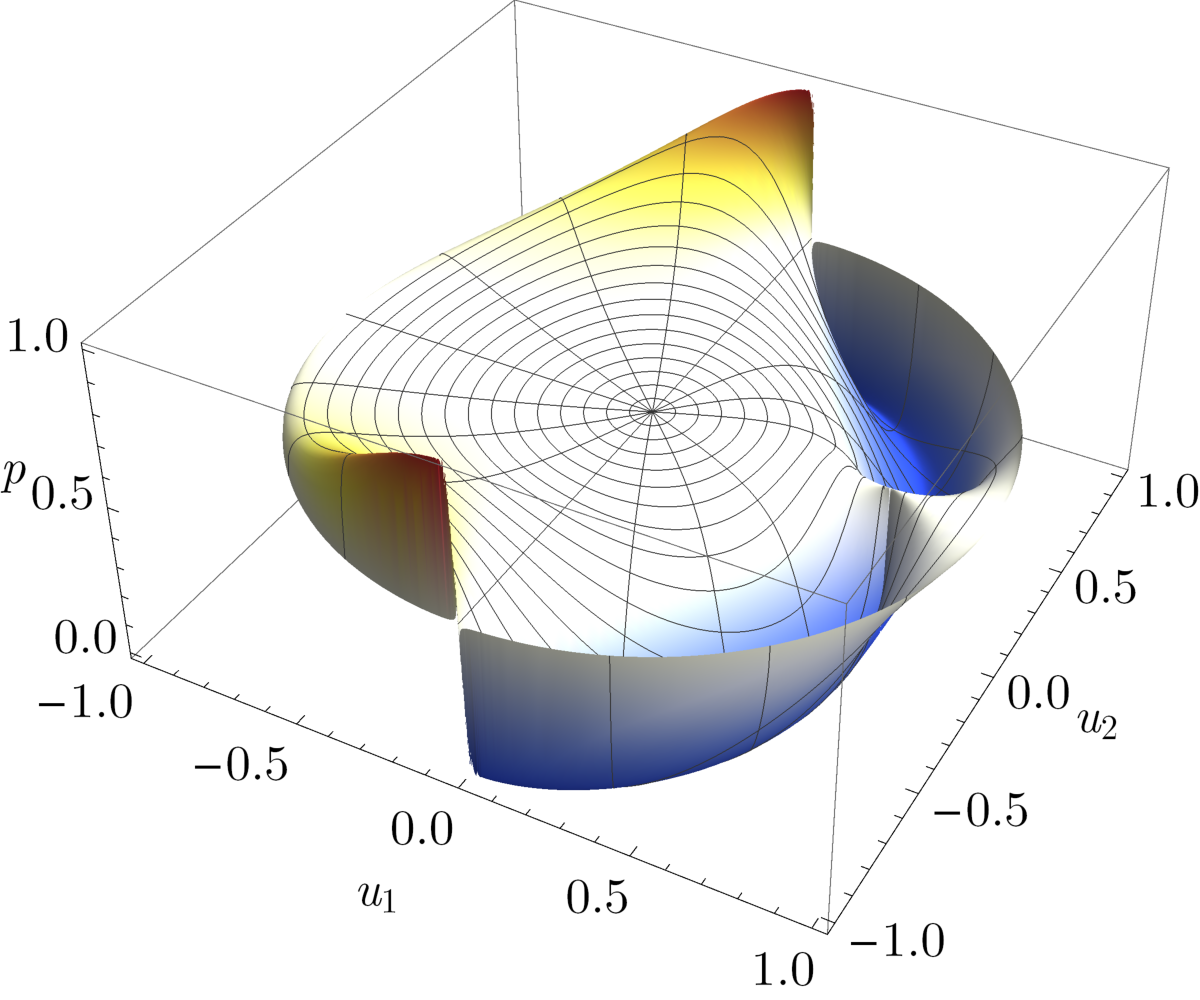
\includegraphics[width=.5\linewidth]{projProbLandscape_2steps_allreal2.pdf}
	\caption{
		Probability given by~\cref{eq:proj_prob_2steps} plotted against $u_1$ and $u_2$, for the special case of $u_1, u_2 \in \RR$.
	}
	\label{fig:proj_prob_landscape_plot3d}
\end{figure}
\begin{figure}[tb]
	\centering
	\begin{tikzpicture}
		\node (img) {\includegraphics[width=.7\columnwidth]%
			{projProbLandscape_2steps_allreal_slices}
		};
		% \node [overlay] (x-axis) at (-.45, -2.4) {\scalebox{1.2}{$u_2$}};
		% \node [overlay] (x-axis) at (-.2, 2.3) {\scalebox{1.2}{$p$}};
	\end{tikzpicture}
	\caption{
		Probability given by~\cref{eq:proj_prob_2steps} plotted against $u_2$, for various choices of $u_1$.
		Each line corresponds to a slice taken from \cref{fig:proj_prob_landscape_plot3d}.}
	\label{fig:proj_prob_landscape_slices}
\end{figure}
\begin{figure}[tb]
	\centering
	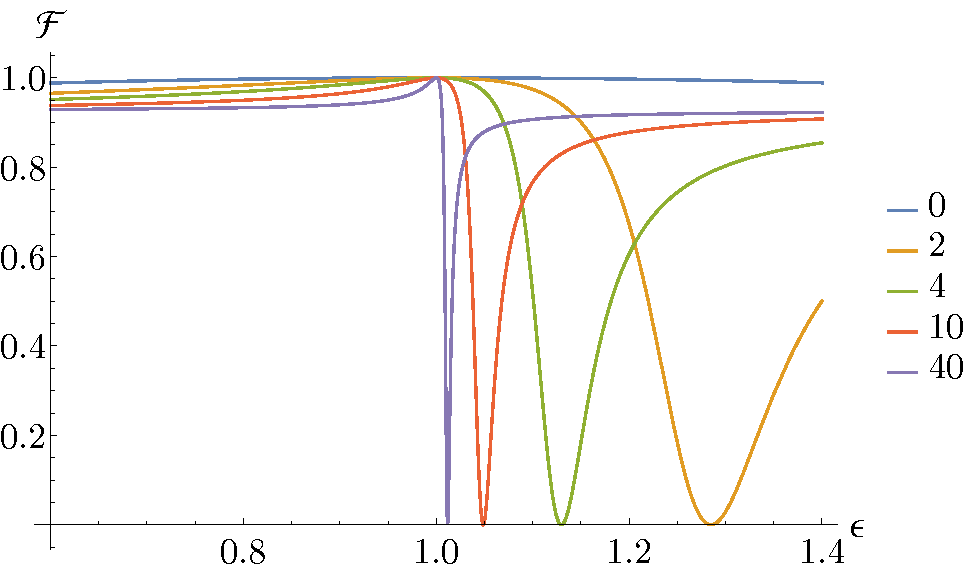
\includegraphics[width=.5\linewidth]{fidelityVsEpsVaryingD_2steps.pdf}
	\caption{
		Fidelity vs a relative change of the value of a coin parameter, for different values of $d_I$.
		Starting from \cref{eq:QWs:state_degenerate_case}, we use as target state the normalised vector
		$\bs u = N (0.5 i, 0.2, 0.5 i)$, and for various values of $d_I$ we compute the coin parameters generating the full state shown in \cref{eq:QWs:state_degenerate_case}.
		We then take a single coin parameter, the parameter $\theta$ in the first step, and substitute it with $\epsilon \theta$, plotting the resulting fidelity between target and generated states as a function of $\epsilon$.
		Larger values of $d_I$ clearly correspond to higher instability.
	}
	\label{fig:fid_vs_eps_varying_d}
\end{figure}

\subsection{Numerical solution of reachability conditions}
\label{sec:QWs:numerical_solution_reachability_conditions}

While, as shown in~\cref{sec:QWs:analytical_sol_2steps}, the $n=2$ case can be fully explored analytically, this is significantly more complicated for larger numbers of steps. Nonetheless,~\cref{eq:QWs:conditions_for_ds} can still be tackled, albeit numerically, for $n=2,3,4,5$.
In this section, we present the results of doing so for a number of random target states sampled uniformly at random.
\Cref{eq:QWs:conditions_for_ds} gives different numbers of solutions for different target states and number of steps:
there is always a single solution for $2$ steps, two or four solutions for $3$ steps, $3, 5, 7$ or $9$ solutions for $4$ steps, and $6, 8, 10, 12, 14$ or $16$ solutions for $5$ steps.
Different solutions for the same target state correspond to different dynamics before the projection, and therefore different projection probabilities.
This can be seen in~\cref{fig:minmax_probabilities}, where we report maximum and minimum projection probabilities for each randomly generated target state.
These results highlight the advantages of solving~\cref{eq:QWs:conditions_for_ds}: having access to the whole set of solutions, we can choose the more convenient one in terms of projection probability.
Moreover, having access to the various solutions generating a given target state, we can study their stability properties.
As shown in~\cref{fig:stabilities_5steps}, a general trend is that sets of coin parameters associated to smaller projection probabilities are also less stable, in the sense that a small perturbation of a coin parameter can lead to a state significantly different than the target one.
As an example, we can use this method to generate a balanced superposition over $4$ sites (using therefore $3$ steps): $\ket\phi = (1, 1, 1, 1) / 2$.
This results in two solutions for the $d$: $\bs d = (-i, 1+i)/2$ and $\bs d = (i, 1 - i)/2$,
corresponding to the full states
\begin{equation*}
\begin{split}
	\frac{1}{2}\Big(
		&\ket{1,\uparrow} + 
		(1 \mp i) \ket{2,\uparrow} \pm i \ket{2, \downarrow} \\
		&\quad \pm i \ket{3, \uparrow} + (1 \mp i) \ket{3, \downarrow} +
		\ket{4, \downarrow}
	\Big),
\end{split}
\end{equation*}
which both result in a projection probability over $\ket+$ of 1/4.
The same procedure applied to a balanced superposition over 6 sites (5 steps) results in 6 solutions, 2 of which with real $\bs d$ and projection probability $\simeq 0.145$, and the other 4 with complex $\bs d$ and projections probabilities of 1/6.
It is worth noting that while the projection probabilities over balanced superpositions over $n$ sites seem to vanish with $1/2n$, a simple phase change of an element can radically change this probability.
As an example, again the case of 6 sites, if the target state is instead $\ket\phi \simeq (1,1,1,1,1,-1)$ the maximum projection probability becomes $\simeq 0.35$.
The stability of the above solutions for balanced states when a small perturbation is applied to the coin parameters is shown in \cref{fig:stabilities_3and5steps_balanced_target}.


\begin{figure}[]
    \centering
    \begin{minipage}[b]{0.5\textwidth}
        \begin{tikzpicture}
            \node (img) {\includegraphics[width=\columnwidth]%
                {projectionProbabilities_2steps_20000states_histogram40binsProbability}
            };
            \node [overlay] (x-axis) at (3.6, -2.6) {\scalebox{1.2}{$p$}};
            \node [overlay] at (0, 2) {\fbox{2 steps}};
        \end{tikzpicture}
    \end{minipage}%
    \begin{minipage}[b]{0.5\textwidth}
        \begin{tikzpicture}
            \node (img) {\includegraphics[width=\columnwidth]%
                {minMaxProjectionProbabilities_3steps_20000states_histogram40binsProbability}
            };
            \node [overlay] (x-axis) at (4, -2.6) {\scalebox{1.2}{$p$}};
            \node [overlay] at (.2, 2) {\fbox{3 steps}};
        \end{tikzpicture}
    \end{minipage}
    \begin{minipage}[b]{0.5\textwidth}
        \begin{tikzpicture}
            \node (img) {\includegraphics[width=\columnwidth]%
                {minMaxProjectionProbabilities_4steps_20000states_histogram40binsProbability}
            };
            \node [overlay] (x-axis) at (4.2, -2.6) {\scalebox{1.2}{$p$}};
            \node [overlay] at (0, 2) {\fbox{4 steps}};
        \end{tikzpicture}
    \end{minipage}%
    \begin{minipage}[b]{0.5\textwidth}
        \begin{tikzpicture}
            \node (img) {\includegraphics[width=\columnwidth]%
                {minMaxProjectionProbabilities_5steps_6000states_histogram40binsProbability}
            };
            \node [overlay] (x-axis) at (4, -2.6    ) {\scalebox{1.2}{$p$}};
            \node [overlay] at (0, 2) {\fbox{5\,\, steps}};
        \end{tikzpicture}
    \end{minipage}
    \caption{
        Distribution of projection probabilities computed 1) solving~\cref{eq:QWs:conditions_for_ds} for the parameters $d_i$,
        2) computing the projection probabilities associated to each full state given by one such solution set, and
        3) picking the solution set for the $\{d_i\}$ associated to lowest and highest projection probabilities.
        The shown data is for the cases of 2, 3, 4 and 5 steps.
        For 2, 3 and 4 steps the data shows the distribution of probabilities from a sample set of 20000 target states, drawn according to the uniform Haar measure over the set of target states.
        For 5 steps only 6000 states were used (being this case much more computationally expensive).
        On the $y$-axis is shown the fraction of target states in a given bin.
    }
    \label{fig:minmax_probabilities}
\end{figure}

\begin{figure}[tbp]
    \centering
    \begin{minipage}[b]{0.5\textwidth}
        \includegraphics[width=\columnwidth]
            {{fidVsParameters_5stepsAnalytical_100thState_prob0.00137738}.pdf}
    \end{minipage}%
    \begin{minipage}[b]{0.5\textwidth}
        \includegraphics[width=\columnwidth]
            {{fidVsParameters_5stepsAnalytical_100thState_prob0.00196137}.pdf}
    \end{minipage}
    \begin{minipage}[b]{0.5\textwidth}
        \includegraphics[width=\columnwidth]
            {{fidVsParameters_5stepsAnalytical_100thState_prob0.00360411}.pdf}
    \end{minipage}%
    \begin{minipage}[b]{0.5\textwidth}
        \includegraphics[width=\columnwidth]
            {{fidVsParameters_5stepsAnalytical_100thState_prob0.00379377}.pdf}
    \end{minipage}
    \begin{minipage}[b]{0.5\textwidth}
        \includegraphics[width=\columnwidth]
            {{fidVsParameters_5stepsAnalytical_100thState_prob0.142292}.pdf}
    \end{minipage}%
    \begin{minipage}[b]{0.5\textwidth}
        \includegraphics[width=\columnwidth]
            {{fidVsParameters_5stepsAnalytical_100thState_prob0.398078}.pdf}
    \end{minipage}
    \caption{
        Behaviour of projection probability of the solutions found solving~\cref{eq:QWs:conditions_for_ds} for the target state $\ket\phi \simeq (0.053, -0.078 + 0.603i, -0.524 + 0.189i, -0.302 + 0.363i, 0.182 + 0.099i, 0.042 - 0.224i)$.
        In each of the plots, the final fidelity is plotted against many coin parameters, each time fixing the value of all of them except for one, whose value is changed by an absolute value $\epsilon$ (x-axis).
        The 6 figures correspond to the 6 solutions for this target state, having respectively the projection probabilities:
        $0.0014$ (top left), $0.0020$ (top right),
        $0.0036$ (middle left), $0.0038$ (middle right),
        $0.14$ (bottom left) and $0.398$ (bottom right).
        As clearly illustrated in this case, solutions with low projection probabilities tend to present an higher degree of instability with respect to small changes of the coin parameters.
    }
    \label{fig:stabilities_5steps}
\end{figure}

\begin{figure}[]
    \centering
    \begin{minipage}[b]{0.5\textwidth}
        \begin{tikzpicture}
            \node (img) {\includegraphics[width=\columnwidth]%
                {{fidVsParameters_3stepsBalanced_prob0.25}.pdf}
            };
            \node [overlay] (F) at (-3.8, 2.8) {\scalebox{1.2}{$\mathcal F$}};
        \end{tikzpicture}
    \end{minipage}%
    % \begin{minipage}[b]{0.5\textwidth}
    %   \includegraphics[width=\columnwidth]
    %       {{fidVsParameters_3stepsBalanced_prob0.25}.pdf}
    % \end{minipage}%
    \begin{minipage}[b]{0.5\textwidth}
        \begin{tikzpicture}
            \node (img) {\includegraphics[width=\columnwidth]%
                {{fidVsParameters_5stepsBalanced_prob0.667}.pdf}
            };
            \node [overlay] (F) at (-3.8, 2.8) {\scalebox{1.2}{$\mathcal F$}};
        \end{tikzpicture}
    \end{minipage}
    % \begin{minipage}[b]{\columnwidth}
    %   \includegraphics[width=\columnwidth]
    %       {{fidVsParameters_5stepsBalanced_prob0.667}.pdf}
    % \end{minipage}
    \caption{
        Fidelity varying the various coin parameters for 3 (left) and 5 (right) steps, when the target is the completely balanced superposition over 4 and 6 modes, respectively.
        The variation of the coin parameters is here shown in percentage: the edges of the plots correspond to a variation of 10\% of a single parameter with the others kept fixed at their optimal value.
    }
    \label{fig:stabilities_3and5steps_balanced_target}
\end{figure}

\FloatBarrier
\subsection{Numerical fidelity maximisation}
\label{sec:QWs:numerical_fid_max}

\tmpHeading{A new method is needed for more than $5$ steps}
Solving numerically~\cref{eq:QWs:conditions_for_ds} for more than $5$ steps is computationally difficult, due to the complexity of the resulting system of equations.
We therefore use a different numerical technique for higher numbers of steps:
we write the fidelity for a given target state as a function of the coin parameters, and find the set of parameters maximizing such fidelity using a numerical optimisation algorithm.
We manage in this way to find solutions for up to $20$ steps much more efficiently than we could have done by directly solving~\cref{eq:QWs:conditions_for_ds}.
% Furthermore, this method eases the study of different final projections, and allows to include the parameters of the projection itself in the optimisation.

\tmpHeading{How we used the optimisation algorithm}
The results of this approach are reported in \cref{fig:prob_histograms_nmaximize}, where we randomly generate a sample of target states, and find through numerical optimisation the set of coin parameters and projections generating them.
It is worth noting that in this procedure we fixed the maximum number of iterations allowed for the maximisation, not the precision with which the final fidelities are to be found.
This is done for the sake of efficiency, as some solutions are found to be more numerically unstable and hard to obtain with very high precisions through numerical optimisation.

\tmpHeading{Results}
As a consequence, as reported in \cref{fig:prob_histograms_nmaximize}, some of the solutions are achieved with relatively low fidelities.
\Cref{fig:prob_histograms_nmaximize} also hints at a correlation between the more numerically unstable solutions and low projection probabilities:
almost all of the solutions that were reached with non-optimal fidelities (that is, fidelity less than 0.99) were also found to correspond to low projection probabilities.
This is consistent with the intuition provided by \cref{fig:stabilities_5steps},
that the lower probability solutions are more unstable with respect to variations of the coin parameters.
\Cref{fig:prob_histograms_nmaximize} shows that in $\sim$90\% (85\%) of the sampled instances we obtain strategies to generate, after 15 (20) steps, states with $p > 0.02$ and $\mathcal F > 0.99$.
% Given the results of~\cref{fig:minmax_probabilities,fig:prob_histograms_nmaximize},
% we believe that this can be sensibly improved by tuning the algorithm.
It is worth noting that --- given the sharp difference between minimum and maximum probabilities reported in \cref{fig:minmax_probabilities}, and the above reasoning substantiated by \cref{fig:fid_vs_eps_varying_d,fig:prob_histograms_nmaximize} ---
% there are strong reasons to believe that even better results can be obtained by properly fine-tuning the optimisation algorithm.
there are strong reasons to believe that almost all target states can be achieved with both high fidelities and probabilities,
by properly fine-tuning the optimisation algorithm.

\begin{figure}[]
    \centering
    \begin{minipage}[b]{0.5\textwidth}
        \begin{tikzpicture}
            \node (img) {\includegraphics[width=\columnwidth]%
                {probsHistogram_15steps_manyThresholds}
            };
            \node [overlay] (x-axis) at (3.8, -2.8) {\scalebox{1.2}{$p$}};
            \node [overlay] at (0, 2) {\fbox{15 steps}};
        \end{tikzpicture}
    \end{minipage}%
    \begin{minipage}[b]{0.5\textwidth}
        \begin{tikzpicture}
            \node (img) {\includegraphics[width=\columnwidth]%
                {probsHistogram_20steps_manyThresholds}
            };
            \node [overlay] (x-axis) at (4, -2.8) {\scalebox{1.2}{$p$}};
            \node [overlay] at (.2, 2) {\fbox{20 steps}};
        \end{tikzpicture}
    \end{minipage}
    \caption{
        Distribution of projection probabilities for randomly sampled states, computed with the numerical maximisation described in~\cref{sec:QWs:numerical_fid_max}.
        Both plots show the probabilities associated to a set of 3000 target states sampled from the uniform Haar distribution, for 15 and 20 steps.
        The light orange (upper) histograms represent the total number of target states found to correspond to a given range of probability.
        Starting from these datasets, we progressively removed the states that were found to reproduce the target states with fidelity less than $1 - 10^{-t}$, for various values of the threshold $t$.
        Light orange, grey, green, dark orange and purple (from top to bottom) histograms correspond to thresholds of respectively $t = 0, 2, 5, 10, 12$ (higher thresholds correspond to only a handful of states and are therefore omitted).
        This data further suggests a connection between the instability of the found solutions with respect to perturbations of the coin parameters, and the projection probability, as already hinted in \cref{fig:stabilities_5steps}:
        it is harder to find numerically with very good fidelity solutions corresponding to low projection probabilities because of their more unstable nature.
        It is also important to note that the solutions shown here are generally not the optimal ones,
        as the optimisation algorithm only seeks to optimize the final fidelity,
        regardless of the corresponding projection probability.
    }
    \label{fig:prob_histograms_nmaximize}
\end{figure}


\section{Conclusions}
\label{sec:QWs:conclusions}
We provided a set of equations characterising the states reachable by a coined \ac{QW} evolution, when letting the coin operation change from step to step.
We then derived a set of conditions characterising the quantum states, spanning only the walker's positions, that are probabilistically reachable after projection of the coin at the end of the walk, discussing both analytical and numerical methods to find the coins generating a target state.
% Finally, we proposed a protocol to experimentally implement the quantum state engineering scheme with linear optics, using orbital and spin angular momentum of a photon to encode spatial and coin degrees of freedom of the walker.
Given the ubiquity of \acp{QW}, our approach should facilitate the engineering of high-dimensional quantum states in a wide range of physical systems.


